\documentclass[11pt]{article}

% ------------------------------------------------------------------
%  GEODE: A Growing Network of Frozen Models
%  Moazzam Abdullah Khan
%  A self-contained introduction to the GEODE system.
%  Compiled with Tectonic (XeTeX), run twice for references.
%
% ------------------------------------------------------------------

\usepackage[margin=2.5cm]{geometry}
\usepackage{amsmath, amssymb}
\usepackage{booktabs}
\usepackage{array}
\usepackage{xcolor}
\usepackage{tikz}
\usetikzlibrary{positioning, arrows.meta, fit}
\usepackage[hidelinks]{hyperref}
\usepackage{microtype}
\DeclareMathOperator{\argmax}{arg\,max}
\DeclareMathOperator{\softmax}{softmax}

\hypersetup{
  pdftitle={GEODE: A Growing Network of Frozen Models},
  pdfauthor={Moazzam Abdullah Khan},
  pdfsubject={An open, verifiable, economically aligned inference network}
}

\title{\bfseries GEODE: A Growing Network of Frozen Models\\[0.4em]
\large Composable contribution, verifiable answers, and payment by measured use}
\author{Moazzam Abdullah Khan}
\date{August 27, 2026}

\begin{document}

\maketitle

\begin{abstract}
Artificial intelligence is in an arms race. Capabilities are built
in secret and deployed in haste. They consolidate in a few hands,
because the race rewards secrecy over safety. GEODE (Generalized
Encoders for Open-Domain Expertise) tries to change that game. It
is a network where anyone can contribute a capability and anyone
can buy answers, priced in Ethereum at market rate. A capability
is a frozen neural network (weights that no longer change) or a
small deterministic program called a primitive. Capabilities are
composable and routable. A contribution can be reused and built
upon by anyone. Every use pays the work beneath it. Payment
follows the measured work that actually served the query. Every
decision is deterministic, replayable, and recorded on a
hash-chained ledger. The wager: collaboration is the fastest path
to advanced AI. Tasks break into smaller composable pieces. They
are cheaper to train and cheaper to run. Competitors build on each
other's work and share the rewards by measured use. A network
anyone can improve compounds faster than central labs that
fossilize under secrecy and intellectual-property protection.
Those who stay outside fall behind. The surplus attention goes to
safety and a rollout that benefits everyone. GEODE claims no new
learning algorithm. Its parts are old and named. Its claim is the
assembly: the composed-codes architecture --- frozen representation
artifacts composed by declaration on a versioned code bus, paid by
measured downstream use.
\end{abstract}

\tableofcontents

% ==================================================================
\section{Introduction}
% ==================================================================

The buildup of artificial intelligence is an arms race. Participants
build capabilities in secret, because secrecy is rewarded. Whoever
ships first captures the returns. Whoever openly publishes the weights 
of their model early hands their work to competitors. The race has 
real costs. Secrecy defeats inspection. Systems ship with less 
understanding than their power warrants. Effort is spent duplicating 
work that already exists. Safety is a cost nobody can afford to pay 
first. And the race is winner-takes-all. The first actor to reach 
general capability would hold a technology too powerful to be governed 
by one hand. Whoever controls the most capable system sets the terms 
on which everyone else has to access intelligence itself. A race whose 
prize is that concentrated cannot be won safely by anyone. It can only be
defused by changing what winning means.

GEODE changes the payoff structure. It does not preach against the
race. Its mechanism is composability and routability. Capabilities
are registered once. Then anyone reuses them and stacks them into
chains~\cite{schick2023}. Every use pays the work beneath it.
This includes uses by competitors building on top. A \emph{task} is
a well-defined piece of work: ``what object is in this picture?'',
``transcribe this recording'', ``forecast this signal one step
ahead''. A \emph{contributor} is anyone who offers a way to do
such tasks. A \emph{user} is anyone who pays for an answer.
Research has always worked this way. Each generation stands on the
shoulders of the previous one. GEODE's wager: collaborative
contribution is the fastest path to advanced AI, and composition
is how it wins. Complex tasks break into smaller, more manageable
pieces. They are cheaper to train and cheaper to run. Competitors
build on top of each other's work and share the rewards according
to use. The effect mirrors the growth of cryptocurrencies.
Innovation happens at the edges, not at the center. Anyone can
make improvements, and everyone is incentivized. Centralized
systems are difficult to change under secrecy and
intellectual-property protection. They fossilize over time.
Anyone who does not take this path loses out in the long run. If
the best return on a capability comes from making it reusable,
self-interest and collaboration point the same direction.

One thing makes it all possible. It is what the name stands for.
GEODE is short for Generalized Encoders for Open-Domain Expertise.
The idea is a registry of frozen encoders. Each maps one kind of
input --- image, audio, text, number series --- into a code space,
and the registry composes them: a head declares a code manifest, an
ordered list of the blocks it reads, and the blocks are
concatenated into one design. CLIP~\cite{clip2021} and
ImageBind~\cite{imagebind2023} built shared embedding spaces for
single models. GEODE extends the idea from single models to a
registry of measured tasks. A task plugs into the registry the way
an application plugs into an operating system. A closed-form head
is fitted on the composed codes. It is measured, priced, and routed
on its own. Nothing beneath it is rebuilt. The registry does not
need to be complete at launch. It needs to be general enough that
new tasks enter as measured additions, not as new foundations.
Where no registered encoder yet covers a data space, the registry
admits another frozen encoder alongside the first, and a head's
manifest simply lists both. Optional closed-form alignment
artifacts --- Procrustes and CCA maps, each one exact solve ---
may be registered as bridges between two blocks; they are measured
and priced per pair, and nothing in the protocol requires one.
The measurements in this paper are the small, real version of that
idea.

Three properties make that payoff structure possible. Everything
else in this paper follows from them.

\begin{itemize}
\item \textbf{Frozen.} Every model in GEODE is a frozen publisher
checkpoint. Its weights are fixed forever. A closed-form fit sits
on top: one direct linear-algebra solve, no iterative training, no
optimizer, no random seed. It is like fitting a straight line
through points, in high dimensions, in one exact computation.
Nothing learns while the network runs. The system reads its models
and never writes them.
\item \textbf{Replayable.} The same declared task and the same
input produce the same routing decisions and the same answer. The
route and the record replay from the hash chain for anyone. The
artifact replays for whoever holds it. The validators check the
replayed results. Weights need not be open for the decision to be
auditable. Every decision is written to a hash-chained ledger.
Records cannot be changed after the fact without breaking the
chain.
\item \textbf{Paid by measured use.} Payments are made in Ethereum
at market rate. They flow to the contributors whose work actually
served the query. They are released gradually over time. A small
share goes to a development fund. Contribution is measured on
held-out data. It is never self-reported.
\end{itemize}

GEODE's ambition is modest and specific. It is to make inference
\emph{inspectable}: you can verify what served you and why. It is
to make inference \emph{accountable}: the people whose work serves
you are the people who get paid. We do not train foundation
models. We do not claim to beat the state of the art. We assemble
established parts --- mixture of experts, classical image codes,
closed-form fits, Bulletproofs, microVMs --- under one measurement
discipline. We test the economic mechanism before it ever governs
real money. Appendix~\ref{app:scenarios} walks those rules through
worked scenarios, actor by actor. Each scenario includes the abuse
attempts and exactly where each one is closed.

One honesty statement organizes the rest of this paper. The
protocol machinery --- the registry, the router, the probes, the
ledger, the settlement --- is built and measured: its rules are
shipped code with sealed tests, and its numbers are held-out
measurements. The generalized-encoder thesis is younger than the
machinery: the fusion, nonlinearity, and breadth measurements in
Section~\ref{sec:measured} support the federated form of the
thesis with measured boundaries --- but the thesis remains an
open experimental program, not a closed claim. Where a
measurement fails, the failure is reported. This paper contains
its own negatives, and the reader should trust the negatives as
much as the positives.

\section{The actors}

The system has few roles. Every rule in this paper attaches to one
of them.

\begin{description}
\item[User.] Anyone who pays for answers. The user declares the
task and pays per unit of work at the posted price.
\item[Contributor.] Anyone who registers a capability. A
capability is an arm (a frozen model) or a primitive (a small
deterministic program). The contributor receives its usage fees,
epoch-vested (an epoch is seven days). Both kinds share one
registration form: an operator
key, a payout address that may differ from it, a price per unit
of work, and a sealed claim. The kinds differ only in who
executes them.
\item[Host.] The address that executes a primitive. The host
earns the host share of its fees. Arms have no separate host
role. Serving the arm is the contributor's own obligation. It is
measured by availability. Hired hardware is a private
arrangement, invisible to the network.
\item[Validator.] A registered party that proposes challenges,
scores answers, and audits other validators. It earns per
accepted challenge.
\item[Reference executor.] A registered party that holds the
sealed artifact and re-runs it inside probed sessions. It is
sampled per session from the artifact's pool under the validator
eligibility rules (activation window, activity floor, tenure). It
is structurally excluded from any artifact that serves the
session. It earns a share of the registered reference-run price.
\item[Librarian.] The single role that appends ledger entries and
executes deterministic registry updates. It is an operator key
during bootstrap. At maturity it is a governance contract with no
human key.
\item[Developer.] The operator of the bootstrap. It holds the
librarian key initially. It ships the bootstrap arms at 80--90\%
of capability and earns hosting fees only. Then it retires per
the headroom rule (Section~\ref{sec:bootstrap}).
\item[Development fund.] The account that receives the 2.5\% share
and the registration fees. Its end state is the zakat rule
(Section~\ref{sec:zakat}).
\end{description}

There is no adjudicator role. Any party may file a dispute with a
deposit. The computation decides guilt. The computation is a
replay of sealed data.

Two actors from outside the system matter as inputs. The
\emph{publisher} provides the frozen checkpoints the arms are
built on. The \emph{benchmark} is the public test suite used as
context. Neither is a GEODE role. Neither is paid by GEODE. A
third outside input is the \emph{registered authority key}: a
government key accepted through the multi-channel rule below. It
can trigger a freeze. It can never burn, and it holds no other
power.

\section{Design principles}

The system's behavior follows from a small set of rules.

\begin{description}
\item[Frozen.] Publisher checkpoints, fixed dictionaries, and
closed-form heads. No component changes at serve time.
\item[Exact where possible.] The task head is a closed-form ridge
fit. Exactness removes the lottery of random-seed training runs.
\item[Deterministic.] Routing is a deterministic function of the
declared task and the measured capabilities. Determinism makes
replay possible. Replay makes audit possible.
\item[Weights may be private.] Verification rests on frozen
hashes, measured reputation, and replay. It does not rest on
reading weights. Contributors are never required to publish their
artifacts. The private serving path (below) keeps it that way even
at inference time: no party holds the head in plaintext except the
contributor's own host.
\item[Private serving.] No party processes request content except
the user's device and the contributor's serving host, and under
the private path the contributor evaluates only ciphertext: the
device encrypts the input, the host computes the answer on the
ciphertext, the device decrypts. The developer and the network
operator process metadata only --- registry, ledger commitments,
routing, and sampling --- never request content. That separation
is a design invariant, not a policy choice.
\item[Measured, not asserted.] Every capability claim is scored
on held-out data. It is sealed with a content hash. It replays
from the ledger. The discipline is register-before-measuring: a
claim is written down before the measurement that tests it.
\item[Economic-only incentives.] Anti-abuse mechanisms use
prices, delays, and burns. They never use identity checks or
whitelists. Identity data is not collected.
\item[No control surface.] The network has no user, region, or
content selection path. A coercer can point at artifacts, never
at audiences. The only content powers are public-record votes
and authenticated freezes, and their effects are fixed:
suspend, never burn.
\item[Earned, capped votes.] A vote counts only with pedigree ---
the activation window, the activity floor, and verified work. It
weighs only with unclaimed earnings. No identity's weight may
exceed a fixed share of the total.
\item[Humble scope.] Every number in this paper is small-scale
and held-out. We state its limits alongside it.
\end{description}

\section{Our assumptions}\label{sec:assumptions}

The design rests on the assumptions below. Each one is a stated
belief, not a measured fact. Where this paper leans on established
crypto practice, it says so in place. Two examples: paying for
access instead of identity checks, and the limits of majority
honesty.

\begin{enumerate}
\item \textbf{Privacy.} People and institutions will pay for
answers whose processing respects their data. Inputs are not
retained beyond the session. They are never used to train any
component without the user's consent.
\item \textbf{Verifiability.} People and institutions will pay for
answers they can verify. Verification rests on the artifact being
frozen, hash-identified, and reputation-scored. It also rests on
the decision record replaying from the hash chain. None of this
requires weights to be open.
\item \textbf{Composition.} Multiple small models can be linked
and routed into chains. The chains serve more complex tasks
without significant accuracy degradation. A chain $g \circ h$ is
admissible exactly when the output contract of $h$ satisfies the
input contract of $g$, written
$C_{\mathrm{out}}(h) \subseteq C_{\mathrm{in}}(g)$ --- the
outputs of the first stage must be valid inputs for the second.
Where composition does not hold, an arm can be a large deep
network of
the current state of the art. The design does not depend on
either path winning everywhere. The measured routing axes
(Section~\ref{sec:measured}) support the composition path's
plumbing. Two full-scale multi-encoder fusion cells are now
measured. The first --- multi-scale codes plus DINOv2 features
upscaled from $32\times32$ --- is a negative for both plain
concatenation and CCA alignment, with the upscaling confound
registered rather than hidden. The second, on a clean cell where
both blocks carry signal (the DINOv2 block re-extracted at native
resolution), reverses the concatenation reading: the fused design
more than doubles the single encoder ($0.548$ vs $0.242$), while
CCA alignment still loses to raw concatenation ($0.511$).
Concatenation on the code manifest is the load-bearing fusion
form; alignment bridges are optional, measured per pair. Both
outcomes are published.
\end{enumerate}

\section{The architecture}

\subsection{The system as a black box}

From the outside, GEODE takes two things in and gives one thing out.

\begin{itemize}
\item \textbf{In: a task description.} A declaration of the kind of
work. It states the input type (image, audio, text) and the
output type (class label, transcript, number). It also states a
small set of fixed attributes. Each attribute comes from a short
allowed list, never free text. An \emph{axis} is a measured task
type: input type, output type, metric, and a published quality
floor, fixed together. The axis metric is per-kind accuracy,
pass@$k$, or word-error rate, each multiplied by the artifact's
measured coverage --- the share of inputs it answers rather than
refuses. A score without a coverage figure is not routable: an
arm answering a fifth of inputs at high accuracy would otherwise
outrank an arm answering everything at lower accuracy, and users
routed to it would receive an abstention most of the time. The
routing mode is
best-value or best-quality. Optional fields cap the unit price
and the total spend. The task is declared with every request. The
system never guesses it.
\item \textbf{In: the sample.} The data to process: the picture,
the recording, the sentence.
\item \textbf{Out: a typed answer with a confidence --- or an
abstention.} The system prefers no answer to a wrong or unsafe
one. It says so. This is the selective-classification stance
of~\cite{geifman2017}. Either way, the decision is recorded. The
answer carries a tag: the artifact that produced it. That
artifact's fingerprint --- what it accepts and what it produces ---
lets the next stage of a chain route onward.
\end{itemize}

The equations in this paper are shorthand for the sentences
around them. Every symbol is explained in words beside it, and
no rule in the system depends on the reader solving any of them.

On a classification axis with a closed-form head, the compute
path is, in symbols, four operations. A frozen encoder maps the
input to a code vector
\begin{equation}
z = f(x) \in \mathbb{R}^d.
\end{equation}
The sealed head scores the $C$ classes of the declared task as a
fixed sum of products,
\begin{equation}
s = W^\top z, \qquad W \in \mathbb{R}^{d \times C},
\end{equation}
the answer is the top-scoring class (the entry of $s$ with the
largest value),
\begin{equation}
\hat y = \argmax_{j \in [C]} s_j,
\end{equation}
and confidence is returned as a coarse bucket, never the raw
number: the winning class's softmax margin is compared against
the artifact's registered bucket edges and the answer carries
only the predicted class and the bucket index,
\begin{equation}
\kappa(x) = \softmax(s)_{\hat y} - \max_{j \neq \hat y} \softmax(s)_j, \qquad
b = \text{bucket}(\kappa(x)),
\end{equation}
The edges are part of the sealed artifact, so the bucketing
replays exactly. The raw margin and the score vector never leave
the serving host: with a public trunk, a margin-annotated answer
stream would let a buyer solve for the head as a linear system
in $d \cdot C$ unknowns; the bucket leaves only coarse
information, and the extraction-cost analysis in
Section~\ref{sec:measured} prices what remains.
The capability abstains whenever $\kappa(x) < \tau$, the axis's
registered margin threshold --- a floor each axis publishes.
Number and transcript outputs are
read out of the same vector through the task's registered
decoder; the four-step form is unchanged.

The contract check enforces the agreement. A sample that does not
match the declared task is rejected, not interpreted.

Verification does not require open weights. The user knows three
things about the capability. It is frozen. It cannot change under
them. Its hash ties it to its record. Its reputation is published
as measured held-out scores. How does the user know the
computation was done correctly? How does the user know their data
stays private? In layers.

The head is a fixed sum of products: the answer is the class
with the largest score, $\hat y = \argmax_j (W^\top z)_j$.
Whoever computes it attaches
a Bulletproofs-style argument. The argument proves that the
reported answer is exactly what the sealed head computes. The
verifier checks the proof at a fraction of the cost of redoing the
computation. The proof reveals nothing about the input. This is
verification without disclosure.

The deep encoder is not yet provable. The reason is speed, not
mathematics. Proving a large network is possible today. It costs
orders of magnitude more than serving. The design deliberately
does not depend on it. This is an honest boundary.

The encoder is a frozen checkpoint. A substituted model is caught
probabilistically. A fraction of sessions is answered twice ---
the shadow probe --- by the serving capability and by a reference
execution of the sealed artifact. The probed contributor pays for
the reference run. The
answers must match exactly. The serving host commits its answer
before it learns whether the session is probed. There is no way
to be honest only when watched.

The user's input enters no public record. The ledger records a
commitment to the answer --- its hash with a fresh nonce --- and
the meter, never the answer itself. The commitment form closes
the transcript-axis exposure: there the answer is the content of
the sample, and a commitment to it publishes no content. The
opening exists only inside the sealed replay environment, where a
dispute is settled. The data contract: inputs are not retained beyond the
session. Codes are not retained either. A code is the encoder's
compact numeric summary of an input, and it can be inverted back
toward the input by a feature-inversion attack. Neither inputs
nor codes are ever used to train any component without the
user's consent.

\subsection{The pipeline}

Inside, one input walks one path. First, an input guard rejects
inputs outside the known input space. Then the contract check
runs. A frozen encoder turns the input into a code vector. A code
vector is a compact numeric summary of the input. The closed-form
head turns the code into the answer. An output contract checks the
answer's type and attaches confidence.

Standing services surround this pipeline. The registry lists the
admitted capabilities. The router picks the capability for the
declared task. The guards enforce the contracts. The ledger
records every decision.

\begin{figure}[t]
\centering
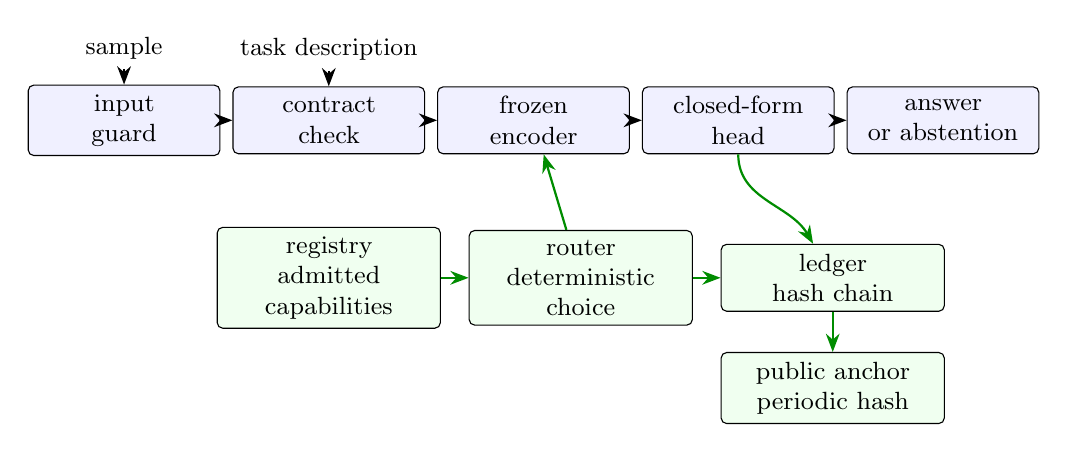
\begin{tikzpicture}[
  font=\small,
  box/.style={draw, rounded corners=2pt, minimum height=8.5mm,
              text width=2.2cm, align=center, fill=blue!6},
  serv/.style={draw, rounded corners=2pt, minimum height=8.5mm,
               text width=2.6cm, align=center, fill=green!6},
  arr/.style={-{Stealth}, thick},
  sarr/.style={-{Stealth}, thick, green!55!black}
]
% pipeline row
\node[box] (guard) at (0,0) {input\\guard};
\node[box] (contract) at (2.6,0) {contract\\check};
\node[box] (encoder) at (5.2,0) {frozen\\encoder};
\node[box] (fit) at (7.8,0) {closed-form\\head};
\node[box] (out) at (10.4,0) {answer\\or abstention};
\draw[arr] (guard) -- (contract);
\draw[arr] (contract) -- (encoder);
\draw[arr] (encoder) -- (fit);
\draw[arr] (fit) -- (out);
\node[above=2mm of guard] (sample) {sample};
\node[above=2mm of contract] (task) {task description};
\draw[arr] (sample) -- (guard);
\draw[arr] (task) -- (contract);
% services row
\node[serv] (registry) at (2.6,-2.0) {registry\\admitted capabilities};
\node[serv] (router) at (5.8,-2.0) {router\\deterministic choice};
\node[serv] (ledger) at (9.0,-2.0) {ledger\\hash chain};
\draw[sarr] (registry) -- (router);
\draw[sarr] (router) -- (encoder);
\draw[sarr] (router) -- (ledger);
\draw[sarr] (fit) to[out=-90, in=120] (ledger);
\node[serv] (anchor) at (9.0,-3.4) {public anchor\\periodic hash};
\draw[sarr] (ledger) -- (anchor);
\end{tikzpicture}
\caption{The GEODE architecture. The pipeline across the top
(blue) turns a sample into an answer; the standing services
beneath (green) select, record, and anchor every decision.}
\label{fig:arch}
\end{figure}

\begin{figure}[t]
\centering
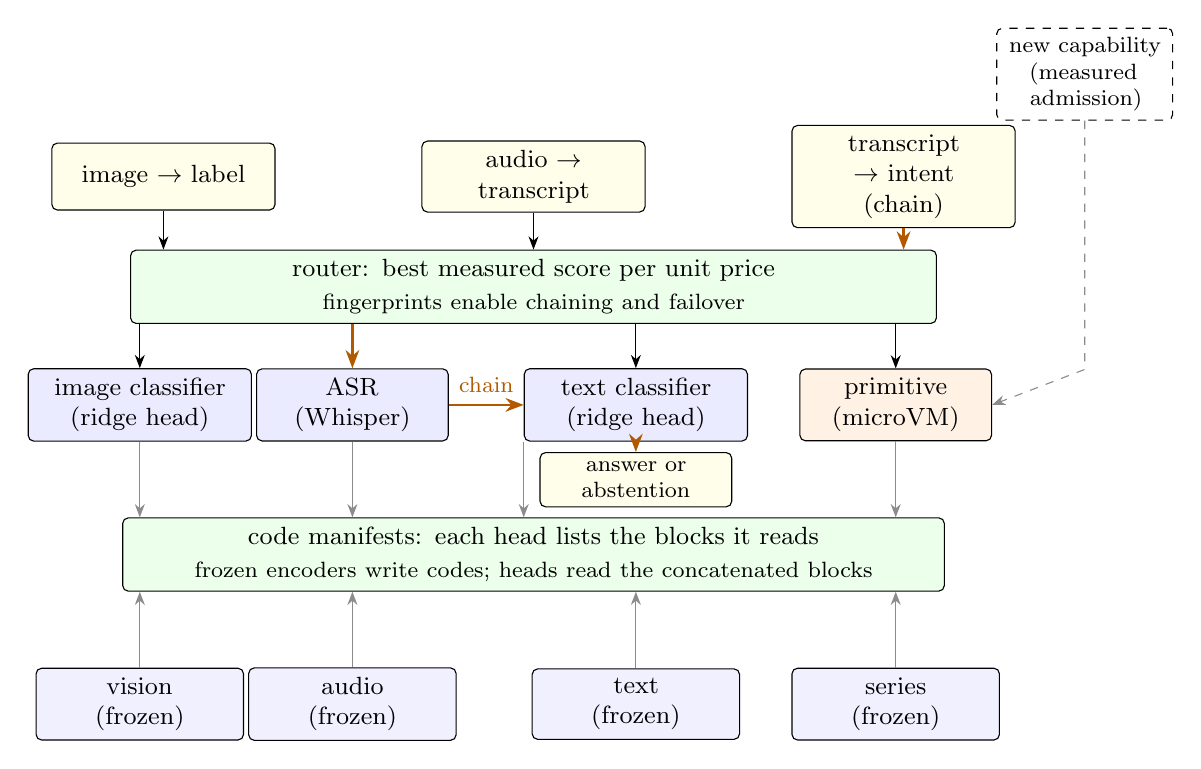
\begin{tikzpicture}[
  font=\small,
  task/.style={draw, rounded corners=2pt, minimum height=0.85cm,
               text width=2.6cm, align=center, fill=yellow!8},
  ans/.style={draw, rounded corners=2pt, minimum height=0.6cm,
              text width=2.2cm, align=center, fill=yellow!8,
              font=\footnotesize},
  serv/.style={draw, rounded corners=2pt, minimum height=0.8cm,
               text width=10.0cm, align=center, fill=green!8},
  arm/.style={draw, rounded corners=2pt, minimum height=0.9cm,
              text width=2.6cm, align=center, fill=blue!8},
  prim/.style={draw, rounded corners=2pt, minimum height=0.9cm,
               text width=2.2cm, align=center, fill=orange!10},
  enc/.style={draw, rounded corners=2pt, minimum height=0.8cm,
              text width=2.4cm, align=center, fill=blue!6},
  arr/.style={-{Stealth}, thin},
  garr/.style={-{Stealth}, thin, black!45},
  chain/.style={-{Stealth}, thick, orange!70!black}
]
% tasks
\node[task] (t1) at (-4.7,3.4) {image $\to$ label};
\node[task] (t2) at (0,3.4) {audio $\to$ transcript};
\node[task] (t3) at (4.7,3.4) {transcript $\to$ intent\\(chain)};
% growth of the network
\node[draw, dashed, rounded corners=2pt, minimum height=0.85cm,
      text width=2.0cm, align=center, fill=white,
      font=\footnotesize] (g) at (7.0,4.7) {new capability\\(measured admission)};
% router
\node[serv] (r) at (0,2.0) {router: best measured score per unit price\\[1pt]
      {\footnotesize fingerprints enable chaining and failover}};
% capabilities
\node[arm] (c1) at (-5.0,0.5) {image classifier\\(ridge head)};
\node[arm, text width=2.2cm] (c2) at (-2.3,0.5) {ASR\\(Whisper)};
\node[arm] (c3) at (1.3,0.5) {text classifier\\(ridge head)};
\node[prim] (c4) at (4.6,0.5) {primitive\\(microVM)};
% answer of the chain
\node[ans] (a) at (1.3,-0.45) {answer or\\abstention};
% shared code space
\node[draw, rounded corners=2pt, fill=green!8, align=center,
      minimum height=0.85cm, text width=10.2cm] (s) at (0,-1.4)
      {code manifests: each head lists the blocks it reads\\[1pt]
       {\footnotesize frozen encoders write codes; heads read the concatenated blocks}};
% encoders
\node[enc] (e1) at (-5.0,-3.3) {vision\\(frozen)};
\node[enc] (e2) at (-2.3,-3.3) {audio\\(frozen)};
\node[enc] (e3) at (1.3,-3.3) {text\\(frozen)};
\node[enc] (e4) at (4.6,-3.3) {series\\(frozen)};
% tasks -> router
\draw[arr] (t1.south) -- (t1 |- r.north);
\draw[arr] (t2.south) -- (t2 |- r.north);
\draw[chain] (t3.south) -- (t3 |- r.north);
% growth: measured admission joins the network
\draw[garr, dashed] (g.south) -- (7.0,0.95) -- (c4.east);
% router -> capabilities (the chain picks ASR)
\draw[arr] (c1 |- r.south) -- (c1.north);
\draw[chain] (c2 |- r.south) -- (c2.north);
\draw[arr] (c3 |- r.south) -- (c3.north);
\draw[arr] (c4 |- r.south) -- (c4.north);
% capabilities read codes from the space
\draw[garr] (c1.south) -- (c1 |- s.north);
\draw[garr] (c2.south) -- (c2 |- s.north);
\draw[garr] (c3.south west) -- (c3.south west |- s.north);
\draw[garr] (c4.south) -- (c4 |- s.north);
% encoders write codes into the space
\draw[garr] (e1.north) -- (e1 |- s.south);
\draw[garr] (e2.north) -- (e2 |- s.south);
\draw[garr] (e3.north) -- (e3 |- s.south);
\draw[garr] (e4.north) -- (e4 |- s.south);
% the chain: ASR output becomes the next stage's input
\draw[chain] (c2.east) -- (c3.west);
\draw[chain] (c3.south) -- (a.north);
\node[font=\footnotesize, orange!70!black] at (-0.6,0.75) {chain};
\end{tikzpicture}
\caption{The network view. Frozen encoders (bottom row) each write
one modality's codes; a head's code manifest lists the blocks it
reads, and the blocks are concatenated into one design. Admitted
capabilities --- arms with closed-form heads, primitives in
microVMs --- answer tasks. The router picks one capability per
declared task. The orange path shows a chain: transcribe audio,
then classify intent, each stage's output satisfying the next
stage's input contract. New capabilities join through measured
admission (dashed).}
\label{fig:network}
\end{figure}

\subsection{The registry and the router}

Admission is by measurement.
\begin{itemize}
\item A submitted registration --- arm or primitive --- passes
quality gates on held-out data. The claim is sealed before
evaluation. This is commit-reveal. A bad result cannot be
re-described after the fact.
\item Quality is measured and sealed. The market prices only the
cost side. A low posted price cannot buy a better score. A high
one cannot claim it.
\item New tasks grow the registry the same way. A measured task
node appends its descriptor and fingerprint to the capability
map. The capability map is the registry's index of what each
capability can do. The extension follows a deterministic rule.
\item Feature blocks are versioned artifacts on a code bus: each
registered encoder extraction carries an encoder version, an
extraction version, a preprocessing version, and a content
digest. A head declares a code manifest --- an ordered list of
the blocks it reads --- and the head is replayable exactly when
its manifest resolves. A version that does not resolve is a
refusal, never a silent default. A new trunk is therefore a new
bus entry, not a registry invalidation: old heads keep resolving
their manifests, and new heads may read old and new blocks
together.
\item The librarian executes these updates as a clerk. It files
the sealed measurement. The rule decides. The key never admits or
extends on its own discretion.
\end{itemize}
Routing is deterministic
(Figure~\ref{fig:network}).
\begin{itemize}
\item The router ranks qualified capabilities by quality per
expected charge: the measured score divided by the posted unit
price and by the expected unit count of the axis's reference
workload. The score is the axis metric oriented so that higher
is better: accuracy, pass@$k$, or inverted word-error rate.
Only capabilities that passed the axis's admission verdict are
considered. A capability that pads its output pays for it here:
bloat inflates the expected charge and lowers the ranking by
exactly that factor. The discipline descends from
mixture-of-experts routing~\cite{shazeer2017,fedus2022}.
Replacing the learned gate with a fixed rule is itself
established prior art: hash-based routing~\cite{roller2021} and
COMET's fixed random projection with a winner-take-all
cap~\cite{shaier2025} route without a trainable gate. What
GEODE adds is that the fixed rule is public and replayable, and
ranks independently registered frozen artifacts by measured
quality per expected charge.
\item The route is a weighted lottery over the top five, with
weights equal to the ranking. It is not winner-take-all: every
qualified capability in the top five keeps a share of traffic
in proportion to its ranking, and the winners' pool mates form
the failover chain in rank order. A newcomer with a smaller
model and a lower price enters the top five on efficiency, not
on pedigree. On a synthetic sweep of the rule, the strongest
arm held about one third of traffic, an equal-price tie split
evenly, and a two-times price cut roughly doubled an arm's
share. Rank ties resolve by a hash of the artifact and the
anchor, never the bare artifact hash: unknowable at seal time,
deterministic per anchor.
\item A per-axis price floor sits at the reference hosting
cost. Registration below the floor is rejected, and
below-floor prices are never routed. The floor stops a price
race to zero. It does not stop an efficient operator from
pricing at the floor and taking the share that efficiency
earns.
\item A task may declare a best-quality mode. This mode ignores
price. A task may also declare a max unit price. Capabilities
priced above it are not considered.
\item Posted prices are ledger entries. Every route replays
against the price table of its day.
\item If no capability is qualified, the system abstains and says
so.
\end{itemize}

Formally, let $Q(t)$ be the set of admitted capabilities
qualified for task $t$, $s_a$ the held-out score of capability
$a$ on the axis, $p_a$ its posted unit price, and $\bar u_a$ its
expected unit count on the axis's reference workload. The
selection score is the quality per expected charge
\begin{equation}
v_a = \frac{s_a}{p_a \, \bar u_a},
\end{equation}
where an unmeasured $\bar u_a$ counts as one and is flagged as
such. Best-value routing draws the route from the top five
capabilities by $v_a$, each weighted by its own $v_a$, so
capability $a$ is chosen with probability
\begin{equation}
\Pr[a \mid t] = \frac{v_a}{\sum_{b \in T_5} v_b},
\qquad
T_5 = \text{the top five of } Q(t) \text{ by } v_a.
\end{equation}
The draw is seeded by the hash of the anchor, the task, the
registry state, and the task fingerprint: deterministic per
anchor, so every route replays, and unknowable before the
anchor, so no host can farm it. Best-quality routing skips the
lottery and selects $r(t) = \argmax_{a \in Q(t)} s_a$. In words:
best-value routing spreads traffic over the top five in
proportion to quality per expected charge; best-quality routing
picks the single highest measured score. If $Q(t)$ is empty, the
system abstains.

\subsection{The ledger and the anchor}

\begin{itemize}
\item \textbf{The chain.} Every decision --- route, answer,
abstention, payment event --- is appended to a hash-chained
ledger. Entry $i$ commits to its payload and its predecessor:
\begin{equation}
h_i = H\bigl(\mathrm{payload}_i \,\|\, h_{i-1}\bigr),
\end{equation}
with $h_0$ the genesis hash. In words: each link seals its own
contents and the seal of the link before it. Change the content
and the hash changes. No record can be altered without breaking
the chain.
\item \textbf{The librarian.} One role appends entries. It is an
operator key during bootstrap. At maturity it is a governance
contract with no human key.
\item \textbf{The anchor.} By default, the ledger tip is anchored
to Ethereum once per epoch. The cadence grows with traffic,
because the cadence is the rewrite window. During development the
anchor goes to the Sepolia testnet, a public practice chain whose
coins carry no value. On mainnet it goes to Ethereum. The anchor
is a notarized public record.
\item \textbf{Prefix immutability.} A chain whose already-anchored
prefix disagrees with any earlier anchor is invalid outright.
Rewriting between anchors cannot be laundered by a later anchor.
The fork rule applies only to unanchored suffixes. A divergence
inside an anchored prefix is a recorded reason to replace the
librarian.
\item \textbf{Force-inclusion queue.} Any party may post an
entry directly to the settlement contract. The librarian must
incorporate it within one epoch of its posting, or the chain is
invalid. Withholding a rival's registration, a dispute filing, or
a mismatch record therefore invalidates the chain instead of
succeeding silently. The queue is an on-chain inbox contract:
posting locks a deposit, incorporation returns it, and a librarian
that fails returns it to the poster while the unincorporated
entry stays visible --- the chain-invalid state is queryable on
chain, never silent.
\item \textbf{Executable replacement.} The librarian is
replaced when a recorded divergence reason collects endorsements
from at least half of the registered validators; a deterministic
deputy takes over at the next epoch.
\item \textbf{Liveness statistics.} Anchor cadence and
inclusion latency are measured, public statistics. A librarian
that stops anchoring, or sits on the inclusion queue, is visible
to everyone on the ledger, not just to its victims.
\item \textbf{Settlement.} Payments are finalized on Arbitrum One.
Arbitrum One is a rollup. It executes transactions cheaply and
posts a compressed proof of them to Ethereum.
\item \textbf{The asset.} ETH is the native asset of both chains.
Payment and claim stay on one asset with no wrapper.
\end{itemize}

\subsection{Proofs of computation}\label{sec:proofs}

An answer also carries a proof of the computation behind it. The
task head is a closed-form ridge fit. It is a fixed sum of
products. Whoever computes it can prove, with a Bulletproofs-style
inner-product argument, that the reported answer is exactly what
the sealed head computes~\cite{bunz2018}. In symbols, the prover
publishes commitments to the sealed head $W$ and the input's
code $z$ and a compact proof $\pi$ of the inner-product
statement
\begin{equation}
s = W^\top z,
\end{equation}
of size logarithmic in the vector length --- the proof grows
slowly, even as the head grows. In words: the proof vouches that
the answer is exactly the sum of products the sealed head
computes. A verifier checks that proof at a fraction of the cost
of redoing the computation. Two places use these proofs.
\begin{itemize}
\item \textbf{Settlement batches.} Each settlement batch carries a
hash of the proofs of the computations it pays for. That
proof-hash is anchored on-chain with the batch. A payment is tied
to a provable computation, not just a claim.
\item \textbf{The verifier.} Anchoring a proof-hash without
verifying the proof would make it decorative. A sampled, paid
batch-verification step at settlement checks the proofs
themselves. It is a registered, ledger-measured role. An invalid
proof is a ledger-disputable L1 deviation. It is replay-gated. It
burns the unvested promise of whoever submitted it.
\item \textbf{Disputes.} A slash is replay-gated. A filed dispute
re-runs the sealed artifact on sealed data. The re-run is itself
a verifiable measurement. The computation decides guilt.
\end{itemize}

The honest boundary: today the proofs cover the small, exact
components. They cover the closed-form head and the router. They
do not cover the full encoder. Proving a large deep network is
possible in principle. It is active research. Today it costs
orders of magnitude more than serving. It is not a shipped
feature. GEODE claims no novelty in the proof technology itself.

\section{The protocol in detail}

The rules above are restated here at implementation depth. An
independent implementer can rebuild the system from this
description. Where a parameter is adjustable, its adjustment path
is stated with it.

\subsection{The task descriptor}

A task is a declaration of fixed fields.
\begin{itemize}
\item \textbf{Input type}: image, audio, text, or number series.
The input type carries its input contract.
\item \textbf{Output type}: class label, transcript, or number.
The output type carries its type check.
\item \textbf{Axis metric}: per-kind accuracy, pass@$k$, or
word-error rate.
\item \textbf{Unit of work}: derived, never chosen. The input and
output types together determine the unit by the registered table
below.
\item \textbf{Routing mode}: best-value (default) or
best-quality.
\item \textbf{Max unit price} (optional): a per-unit price
ceiling. Capabilities priced above it are not considered.
\item \textbf{Max spend} (optional): a total cap on the session's
charges, in ETH. Serving stops when the remaining cap is less
than one unit. Unspent budget is never charged.
\end{itemize}
The descriptor is content-hashed; its registry identifier is
$\mathrm{id}(\tau) = H(\tau)$ --- a fixed-length digest of the
descriptor's exact contents --- and that digest is the task's
identifier in the registry.

\textbf{How the unit follows from the description.} The unit of
work is a function of the input type and the output type
together. It is not a function of either one alone. It is not a
free field. A registered table maps each admissible pair to its
unit:

\begin{center}
\begin{tabular}{@{}lll@{}}
\toprule
\textbf{Input} & \textbf{Output} & \textbf{Unit} \\
\midrule
image & class label & query \\
text & class label & query \\
number series & number & query \\
audio & transcript & audio second (input duration) \\
text & transcript & token \\
text & audio & audio second (output duration) \\
\emph{any (primitive)} & \emph{any} & execution attempt \\
\bottomrule
\end{tabular}
\end{center}

A pair without a row is not an admissible task until the table is
extended. The extension is a registered rule change, never a
per-task choice. Describing the task fixes the unit. No
registration chooses it. Every registration on the axis prices in
it. The descriptor's hash freezes it.

\subsection{The fingerprint}

A capability's fingerprint encodes what it accepts and produces.
It is the tuple
\begin{equation}
F(A) = \bigl(\tau,\; C_{\mathrm{in}},\; C_{\mathrm{out}},\;
\mathcal{L}\bigr),
\end{equation}
where $\tau$ is the task descriptor, $C_{\mathrm{in}}$ and
$C_{\mathrm{out}}$ the input and output contracts, and
$\mathcal{L}$ the class list --- in words: what task it serves,
what inputs it accepts, what outputs it produces, and which
labels it can emit. Two capabilities with identical
fingerprints are interchangeable on that task. That makes
composition and failover mechanical. The fingerprint is computed
from the sealed artifact. It is never computed from a
self-description.

\subsection{The head}

The head is a ridge fit on frozen features. There are $n$
training rows with code matrix $X \in \mathbb{R}^{n \times d}$
and label matrix $Y \in \mathbb{R}^{n \times C}$. For
classification, each row of $Y$ marks the true class with a 1
and the rest with 0. That is a one-hot encoding. The head
minimizes the penalized least-squares objective --- the squared
distance between the head's predictions and the labels, plus a
small penalty $\lambda$ on large weights; the same calculation
as fitting a straight line through points, in high dimensions,
\begin{equation}
\min_{W} \; \| XW - Y \|_F^2 + \lambda \| W \|_F^2,
\end{equation}
whose single exact solution is
\begin{equation}
W = (X^\top X + \lambda I)^{-1} X^\top Y,
\end{equation}
with $\lambda$ a registered regularization parameter. At serve
time a fresh code $z$ is scored by the sum of products
$s = W^\top z$ and answered by the class with the largest
score, $\hat y = \argmax_j s_j$. The
solve has no iterations and no random seed. The solver,
$\lambda$, and the training rows are part of the sealed
artifact. The head replays bit-exactly. It is a closed-form
readout~\cite{belrose2023} in one exact solve.

\subsection{Registration proofs}

\begin{itemize}
\item \textbf{Contributors.} At registration the contributor
submits the artifact hash, the fingerprint, and a contract proof.
The proof is a compact Bulletproofs-style
argument~\cite{bunz2018}. It proves that the sealed head
satisfies the declared output contract on a sampled set of
ledger-registered reference codes. A reference code is the frozen
encoder's output on a reference input, and the encoder run that
produces each code is itself registered in the ledger, so the
code is a recorded datum, not a raw input. For each sampled
reference code $z_i$, the proof attests
\begin{equation}
y_i = \mathrm{decode}\bigl(W^\top z_i\bigr),
\end{equation}
where $\mathrm{decode}$ is the registered readout of the output
contract. In words: the proof vouches, code by code, that what
the sealed head produces on each sampled reference code is what
the contract says it must produce. Proving the encoder run that
made the code is out of scope, by design (next item). The network
verifies the proof. The fingerprint is then a cryptographic
statement about
the artifact.
It is not a self-description.
\item \textbf{The boundary.} The proof covers the head. The head
is the exact, closed-form part. The frozen encoder is verified
differently, by design. The shadow probe, replay, and the
contributor's slashable revenue window cover it. Proof does not.
Proving a large deep network is possible in principle. It costs
orders of magnitude more than serving. It would enter only if a
registered cost trigger fires. The design does not depend on it.
\item \textbf{Validators.} Honesty cannot be proved at
registration. It is bought instead: a fee to enter, a slashable
promise, audits, and burns. Each challenge carries a per-point
commitment. A revealed label can be checked against what was
committed.
\item \textbf{What disputes remain.} Anything still in dispute is
settled by deterministic replay.
\end{itemize}

\subsection{Admission, step by step}

Admission is one procedure for both kinds of contribution. A
primitive's challenges are reference executions. Everything else
is identical.

\begin{enumerate}
\item The contributor submits the artifact hash, the fingerprint,
the descriptor, the contract proof, and the claimed scores.
\item The claim is sealed (commit) before evaluation.
\item Validators score the artifact on the held-out split
(reveal).
\item The verdict compares the measured score against the axis's
published floor.
\item On pass, the artifact is admitted. The registry appends a
public, append-only entry.
\end{enumerate}

\textbf{What the measurement measures.}
\begin{itemize}
\item Contributors train on whatever data they like. The network
does not audit their training data. It measures data the
contributor cannot see.
\item The network holds its own evaluation corpora. They are
collected, held sealed, and never released. Every submission is
scored on splits the contributor never touches.
\item Where a public benchmark is used, the network does not
score on the benchmark's public test split. It holds its own
sealed partition.
\item Splits rotate. A leaked row loses its value.
\item Boundary one: contributor data may overlap the evaluation
data. That is an unearned boost, impossible to rule out.
\item Boundary two: the frozen encoder is a publisher checkpoint.
No one can audit its pretraining history. Publisher numbers are
reproduced as a sanity check only.
\item The developer's own bootstrap arms seal the head's training
rows for bit-exact replay. That is an internal discipline, not a
requirement on contributors.
\end{itemize}

\textbf{Defenses against probing.}
\begin{itemize}
\item Verdicts are aggregate-only. They give one score per axis.
They never give per-row outputs or per-class breakdowns.
\item Scores are reported to bounded precision: four significant
digits. Single-row influence is about one part in the split size.
It sits below that resolution. The exact value stays in the
ledger.
\item Every submission pays the registration fee. Repeated
probing costs money.
\item Residual: probing resistance is a cost barrier, not a
proof.
\end{itemize}

\textbf{Custody.}
\begin{itemize}
\item The evaluation corpora live inside a sealed scoring
environment. Validators submit queries and receive aggregate
scores back. No validator holds rows. Nothing leaves the
environment except aggregate verdicts.
\item Inside the environment the corpus is sharded, so no single
operator key reads the whole corpus at once. A row that leaks out
identifies which shard it came from, and the slash path applies.
\item Shards reshuffle at each rotation. Retired rows are
replaced.
\item The rubric is public. It holds the floors and metrics. Only
the data is secret.
\item Residual: the sealed environment itself is an
infrastructure trust point, and a corrupt majority of validators
is outside the mechanism's reach.
\end{itemize}

\textbf{The challenge layer (overview; specified below).}
\begin{itemize}
\item Validators commit hashes of challenge points. The input is
posed with the expected output hidden. The frozen artifact
answers. The expected outputs are revealed. The answers are
scored.
\item Every step is a ledger entry. The verdict replays for
anyone. The hidden split can never offer that.
\item A correct answer that lands before its challenge's reveal
is structural proof of collusion. Both parties face the slash
path.
\item Challenges use disposable data. Every revealed point is
public thereafter.
\end{itemize}

\subsection{The challenge session}

\textbf{Registration.} A validator registers per task axis. The
form holds an operator key, a payout address that may differ from
it (cold-key hygiene), the axes it serves, and a registration fee.
The entry is append-only in the registry. A validator joins a
sample only after an activation window of two epochs from
registration. It must also be active: it responded to at least
half of its sampled rounds inside the trailing two epochs. A
flood of fresh registrations therefore carries no sampling weight
at admission. The same rule applies in the quorum takedown.

\textbf{Sampling.} An admission has commit hash $c$ on axis $a$.
Each validator in the axis's pool is keyed by
$H(\text{validator id}, b, a, c)$, where $b$ is the first
randomness-beacon round that closes after the commit was frozen
on the ledger (the beacon is defined with the ledger below). The
sampled set
is the first $k$ entries in that key order. Default $k=9$. No one
chooses their judges. The seed postdates the commit and is
produced by a beacon the librarian does not control. The
submitter cannot grind it by re-rolling the seal.

\textbf{Rounds.} Challenges are drawn, not authored. They
come from a registered sealed per-axis corpus under a published
stratified sampling rule: the beacon-seeded draw is stratified by
class share (equal per class unless shares are registered), and
the corpus is committed by Merkle root at axis creation. The
validator's job is to sample, pose, verify, and attest --- never
to choose the exam. Every artifact on the axis is therefore
measured against one fixed population quantity, which is what the
router's score comparison assumes. For each drawn
challenge: (1) commit
$c_j = H(x_j, y_j^*, n_j)$ over the input $x_j$, the expected
output $y_j^*$, and a nonce $n_j$; (2) pose the input; (3) the
frozen artifact answers $\hat y_j$; (4) reveal input, expected
output, nonce; (5) score the agreement --- one if the answer
matches the hidden expected output and zero otherwise,
$a_j = \mathbb{1}[\hat y_j = y_j^*]$, or for a transcript
$a_j = 1 - \mathrm{WER}(\hat y_j, y_j^*)$, one minus the
word-error rate. A challenge is void
unless its input passes the task's input contract and its
revealed output passes the output type check.

\textbf{Verdict.} Let $m_v$ be validator $v$'s count of accepted
challenges and $\bar a_v$ its agreement rate on them. The score
is the quorum-weighted agreement
\begin{equation}
S = \frac{\sum_{v} m_v \, \bar a_v}{\sum_{v} m_v},
\end{equation}
taken over validators that submit accepted challenges. In
words: each validator's agreement counts in proportion to how
many valid challenges it contributed. The artifact passes when
$S$ meets the axis's published floor. A
supermajority of responders must submit accepted challenges. The
default is two-thirds, with a minimum of three.

\textbf{Collusion.} A correct answer whose ledger time precedes
its challenge's reveal is a registered proof of pre-reveal
collusion. Validator and contributor both face the slash path.

\textbf{Audits.} After each session, a fraction of the revealed
challenges is re-labeled independently by two other validators.
The default fraction is one-tenth. The audit work is paid from
the challenge budget at the registry-set rate. Unpaid audit work
would be shirked. A sampled auditor that declines earns a demerit.
A validator whose expected outputs disagree with the audits on a
registered fraction of the audited points burns the unvested
promise and leaves the pool.

\textbf{Availability.} Validators only push entries. There is no
inbound endpoint. The quorum is taken over responders.
Availability is measured as responded rounds over sampled rounds.
Below a registered threshold, the validator is delisted.

\textbf{Payment.} Each accepted challenge is paid from the
contributor's challenge budget at the registry-set per-challenge
fee. The fee is never contributor-set. A contributor-set fee could
double as a bribe. Payments are epoch-vested ($N=4$), pull-claimed,
and docked 2.5\%. They settle in the epoch batch. Nobody is paid
for silence.

\subsection{Failure handling}

\begin{itemize}
\item \textbf{No-shows.} A sampled validator that does not respond
within the round window is absent for that round. The quorum is
taken over responders. If fewer than the minimum respond, the
session fails closed. The default minimum is three. No admission
happens. The unspent budget is returned.
\item \textbf{Void challenges.} A challenge is void if its input
violates the input contract. It is void if its output violates
the type check. It is void if it repeats an already-revealed
point. It is void if it overruns the per-validator quota. Void
challenges score nothing and earn nothing. Repeat voids count as
availability demerits.
\item \textbf{Weight caps.} Every validator's challenges are
capped at $m$ per round. No validator can dominate the verdict by
volume. Quorum weight is proportional to accepted challenges.
\item \textbf{Wrong labels.} A validator whose revealed expected
output disagrees with the independent audit relabeling is
excluded from the session. The score is recomputed without its
challenges. Its fee burns. A repeat offender is delisted.
\item \textbf{Collusion.} A correct answer whose ledger time
precedes its challenge's reveal voids the challenge and slashes
both parties.
\item \textbf{Stalling.} A contributor who does not answer posed
challenges within the window voids them. A session that cannot
reach quorum fails closed. On quorum failure the validator set is
resampled and the unspent budget carries forward: a colluding
minority that bleeds a rival by silence pays for the griefing
itself, and the victim does not pay a second fee. Non-response in
a sampled round counts as a demerit weighted by how close the
session came to quorum.
\item \textbf{Disputes.} Any party may file a dispute with a
deposit and an evidence reference. The deposit is the registered
reference-run price. It is deliberately bounded, so the dispute
right is affordable to any contributor. The computation re-runs
the sealed artifact on the challenged point inside a sealed
replay environment. The disputed input is reproduced only there.
It never enters the public ledger. The outcome is deterministic.
The losing party pays the full replay cost. An upheld dispute
returns the deposit and slashes the wrong party. A rejected
dispute burns the deposit.
\item \textbf{Appeals.} A contributor may demand one full replay
of its session. The replay is deterministic from the ledger. A
replay that reproduces the verdict closes the appeal. The
appellant pays the replay cost. A replay that fails to reproduce
it corrects the verdict and refunds the submission budget.
\item \textbf{Timeouts.} A session runs at most $R$ rounds. The
default is three. At the close, the verdict is computed from
accepted challenges. An unmet quorum fails closed. Unspent budget
is returned.
\item \textbf{Forks.} A ledger fork is two parties holding
different chains. The fork rule reads the verdict from the chain
with the latest Ethereum anchor, over unanchored suffixes only.
A chain whose anchored prefix disagrees with an earlier anchor is
invalid outright. Diverging copies are ignored. A divergence is a
recorded reason to replace the librarian.
\end{itemize}

\subsection{Serving verification}

\textbf{Private serving.} The privacy-critical serving
path is fully homomorphic evaluation of the closed-form head.
The user's device encrypts its input $z$ under the registered
scheme and sends only ciphertext to the contributor's serving
host. The host evaluates the frozen head --- the fixed sum of
products $W^T z + b$, with $W$ never leaving the host --- on the
ciphertext, and returns the encrypted score vector. The device
decrypts and takes the argmax on-device. No server --- nor any
coalition of them --- ever sees $z$, $s$, or the answer, and the
contributor physically cannot farm user vectors. User privacy is
ciphertext-grade: it rests on the scheme's security, not on who
owns any server. No party ever holds $W$ in plaintext except the
contributor's own host, so model privacy is unconditional. The
developer is not a party. Encoder placement is tiered:
phone-class encoders run on the device (the default); quantized
encoders may run on device NPUs where their fp32-equivalence gate
passes; SOTA trunks the device cannot run use the premium tier,
where the device FHE-encrypts the input, the contributor
evaluates the frozen trunk on ciphertext only, and the device
decrypts its own features and continues the protocol above ---
under the head encryption, the trunk and the head are one
ciphertext path. The FHE cost is measured at roughly twenty
seconds per query on one CPU for the head path, parallelizable
across cores and queries, and is priced by the contributor as a
premium; the developer processes no content in any tier.
Clients without on-device compute use the plaintext tier,
disclosed as such.

A contributor could pass admission with one artifact and serve
another. The shadow probe catches this.

\begin{itemize}
\item \textbf{The shadow probe.} A registered fraction $\rho$ of sessions
is answered twice. The default is $\rho=0.05$, timelock-adjustable
upward only: the floor of $0.05$ sits outside ordinary governance
(see security floors).
The serving capability answers once. A reference execution of the
sealed artifact answers once more, on the same session's input.
The two answers must be identical: any
$\hat y_{\mathrm{serve}} \neq \hat y_{\mathrm{ref}}$ is a
deviation. The comparison is live. It is
never against the registration challenge set. A memorizing
lookalike could pass a stored set. It cannot know tomorrow's user
inputs. A relative rate under-samples quiet axes. Every active
axis therefore carries a per-epoch minimum of probed sessions.
The default minimum is one. The detection horizon stays inside
the vesting promise everywhere.
\item \textbf{Behavioural identity.} At admission the
contributor commits to a Merkle root over $f(x)$ on a large
sealed probe set. Each epoch a beacon-seeded fresh slice is
revealed and the serving host must answer it; the answers must
open against the committed root. Locality checks pair each probe
with perturbed neighbours: a stored lookup table answers exact
probes but not their neighbours, while the real artifact answers
both. The mechanism lets a serving host prove behaviour without
distributing weights.
\item \textbf{Identity, not accuracy.} The probe certifies that
the served model \emph{is} the sealed artifact. That is the only
claim a serving-time check can measure. A live sample carries no
label. Accuracy was settled at admission on held-out splits. It
is re-settled whenever an artifact re-registers. Serving the
artifact serves its certified accuracy by construction. The
comparison asks for sameness, never for a correctness percentage.
On a deterministic artifact an honest contributor matches every
probe. The honest bar is match-always. No accuracy floor is
re-levied at serving time. A cheaper model that answers
identically everywhere is the same function and no violation.
The network buys answers, not compute. If a pipeline has benign
nondeterminism, its reference-to-reference divergence is measured
at registration. The match band is set from that. It is a band
around ``the same artifact''. It never licenses the served model
to differ by the artifact's own error rate. Replay rests on a
registered numerics policy: float64 promotion in the head's
solve, pinned kernels, fixed reduction order. Measured: the
canonical CPU oracle reproduces the sealed heads bit-exactly on
its registered configuration, while the same computation under a
different thread configuration diverges in the last bits. The
probe therefore compares margins, never raw bits.
\item \textbf{Commitment, not secrecy.} A session's probe flag is
drawn from the randomness beacon, ordered by the epoch anchor.
The serving host must commit the
hash of its answer before that flag is revealed. A host cannot
know whether a session is probed until its answer is already
bound. The only strategy that passes every probe is to serve the
artifact every time. The reference execution runs inside the
probed session and compares against the committed answer. The
duplicate is discarded with the session. Probe choice need not be
unpredictable. It only needs to come later than the answer.
\item \textbf{A mismatch burns.} A differing answer is a
ledger-disputable deviation. It is replay-gated. It burns the
unvested promise. Repeat offenders are delisted.
\item \textbf{The judge is sampled, not chosen.} Reference
executors register against the artifact they hold. They earn
eligibility the way validators do. There is an activation window
of two epochs from registration. There is an activity floor:
reference runs completed in at least half of their sampled
assignments inside the trailing two epochs. Tenure weight applies
in the sampling. A different key is cheap. A pedigree is not. A
flood of fresh accounts is almost never sampled. Each probed
session samples $k_e$ executors, default two. The sample is a
hash of the randomness-beacon round, the session, and the serving
host's own
answer commit. The judges are unknowable until the host's answer
is already bound. No single executor judges any session alone.
The registered reference-run price is divided among the sampled
set. The probed contributor's dock stays one registered price.
\item \textbf{Who judges the judge.} Every sampled executor
commits its reference answer before any answer is compared. The
commit covers the input's hash. An executor cannot fabricate a
mismatch after seeing the answer. It cannot rubber-stamp a
substitution. Neither party can substitute a different input at
dispute time. Executors that disagree with each other or with the
committed answer are all bound by replay. The disputed input is
reproduced only into the sealed replay environment. The sealed
artifact decides. Whoever it contradicts pays the replay and
burns. Both roles carry the same slashable promise. A dispute is
filed with a deposit set at the registered reference-run price.
The deposit is deliberately bounded, so the dispute right is
affordable to any contributor. The loser pays the full replay
cost. The deviation burn is destroyed, never awarded to anyone.
A false claim has no upside. The disputed session's credit
escrows until the replay settles.
\item \textbf{Why it deters.} Each session is probed with
probability $\rho$, so the number of sessions until a substituted
artifact is first probed is geometric with expectation
$\mathbb{E}[T] = 1/(\rho\delta)$, where $\delta$ is how often the
substitute disagrees with the sealed artifact. A crude knockoff
that differs on every input ($\delta = 1$) is probed within
$1/\rho$ sessions --- twenty on average at the default
five-percent probe rate. A close copy that differs on only 0.5\%
of inputs ($\delta = 0.005$) hides for about 4000 sessions. The
probe therefore deters crude substitution and is weak against
near-copies. A sequential test over the mismatch stream closes
the near-copy case, and it is shipped and measured: at the
registered bounds it convicts a 99.5\%-agreeing substitute at
rate 0.958 within a median 2383 sessions, while falsely
convicting an honest host at rate 0.004. The
contributor's entire revenue window sits inside the vesting
promise. Colluding with a
judge is
no cheaper. Every sampled executor must be corrupted. A
host--executor ring needs a corrupt fraction of the pool raised
to the executor count, not a single fresh key.
\item \textbf{The cost.} The shadow probe is the contributor's
ongoing honesty certificate. Admission sets the precedent: admission costs
the contributor, never the network. The probed session's credit
is docked the registered reference-run price. The price is
divided among the sampled executors who ran the reference
execution. Each sampled executor performs one full reference run.
An executor joins rationally only if its divided share covers
that run, so the registered reference-run price must be at least
$k_e$ times the cost of serving one session. Expected probe
overhead is therefore at least $k_e\rho$ of serving cost --- about
ten percent at the defaults, not five. The confidence knob
($k_e$) and the cost knob are the same number, and the tension is
stated rather than hidden. Anyone holding the sealed artifact can register into
its executor pool. It is a paid, measured role, not a permanent
developer duty. The executor sees the probed input in plaintext
--- a further plaintext point alongside the gateway and the
serving host. The ledger never carries the answer: the answer
entry is a commitment whose opening exists only inside the
sealed replay environment. The same
data contract binds every point: no retention
beyond the session, no training. Probe coverage is itself a
ledger-measured rate. A provider that falls silent is visible.
The governance quorum re-routes the demand to another. The
residual: if every provider stops, detection degrades to disputes
alone. That is a public, measurable state, not a hidden one. The
development fund carries no per-session monitoring line.
\item \textbf{The operative mechanism, per tier.} The probe above
is the operative live-traffic mechanism for artifacts with a
non-empty executor pool --- anyone holding the sealed artifact may
register into it, so the pool is empty only when the contributor
keeps the weights private. For weights-private artifacts on the
plaintext tier, the operative mechanism is behavioural identity:
a fixed, Merkle-committed probe set with locality checks and
behavioural dedup at registration --- not fresh-input probing,
which needs the artifact. The near-copy-on-live-traffic residual
for such artifacts is real and is sized by the bond, not denied.
For the private (FHE) tier, the probe is ciphertext-native: the
host commits the output ciphertext and the executor replays the
homomorphic evaluation on the same ciphertext --- no plaintext
point exists in the probe at all, and the executor pool for a
weights-private FHE contributor is the contributor's own host,
whose evaluation is committed and replayable on the same terms.
Each tier therefore names one operative mechanism, and the
empty-pool case carries its stated residual.
\end{itemize}

\subsection{The ledger}

Entry types: route, answer, abstention, payment, price table, and
registry. Every entry carries its type, its payload, the unit
counts it meters, the previous entry's hash, and its own hash.
The answer entry carries the commitment $H(\text{answer} \|
\text{nonce})$, never the answer. The route entry carries a
Merkle root over the registry state it decided against --- every
score, price, and qualification in force at route time --- so a
route replays as a local check against a committed root instead
of a whole-chain reconstruction.
By default, the tip is anchored to Ethereum once per epoch. The
anchor payload is (tip hash, record count, last record hash).
The anchor is the timing reference. Sampling randomness comes
from elsewhere: a public randomness beacon (drand, or the beacon
chain's RANDAO composed with a verifiable delay function) whose
output the librarian does not produce. Every sample in the
protocol --- probe flags, validator sampling, reference-executor
sampling --- derives from that beacon, composed with the anchor
for ordering. A party that appends ledger entries can therefore
delay a sample's clock but never choose the sample itself.

\subsection{A session, end to end}

A session is one declared task and the samples served under it.
\begin{enumerate}
\item \textbf{Declare} the task.
\item \textbf{Route}: best measured score per unit of posted
price (the axis metric oriented so that higher is better).
\item \textbf{Serve}: the frozen artifact answers.
\item \textbf{Meter}: units counted from the typed answer.
\item \textbf{Cap}: the session stops at the declared maximum
spend, if any. A unit that would exceed it is not served.
\item \textbf{Pay} at the price locked at routing time, for the
units actually served.
\item \textbf{Record}: the ledger entry.
\end{enumerate}
A registered fraction of queries is also answered by a reference
execution of the sealed artifact within the same session. The
answers must match. An abstention consumed the trunk compute: it
is recorded and metered at the registered reduced rate --- half
the unit price --- never free. The boundary-mapping queries that
probe the margin threshold are exactly the queries most likely
to abstain, and they pay for the compute they burn.

\subsection{Settlement batching}

Payments are batched per epoch. At each epoch boundary the
librarian aggregates the session credits into one settlement
transaction on Arbitrum One. The batch payload carries the
proof-hash of the computations it pays for, anchored on-chain
with the batch (Section~\ref{sec:proofs}). A malformed credit is
skipped with a logged event. It never reverts the batch.

\section{Programmable primitives}

A learned arm is not the only kind of contribution. GEODE also
admits \emph{programmable primitives}. A primitive is a small
deterministic program. Examples: memory stores, math engines,
transforms, and later anything anyone writes in a supported
toolkit (Python first). A primitive presents the same interface
as an arm: typed inputs, typed outputs, measured utility, fees by
usage. It is admitted the same way: one registration form, one
validator challenge session, one contributor-set price per unit
of work. A primitive's challenges are reference executions. The
two kinds --- learned arms and programmed primitives --- are
collectively \emph{capabilities}. Once sealed, either kind is
called an \emph{artifact}. Every rule about artifacts applies to
both.

\subsection{The standard library}

A small standard library ships free with the network. The
developer provides it. It is permissively licensed, hash-pinned,
and runs on each contributor's own machine. It earns nothing for
anyone. It is infrastructure, like the road a delivery service
drives on. The development fund maintains it as a public good.

The catalog grows continuously. It launches with, by category:

\begin{itemize}
\item \textbf{Memory.} A count-based variable-order memory over a
token stream: register, backoff lookup, predict-next. It stores a
count table, not weights.
\item \textbf{Math.} Scale, clip, affine transform, L2
normalization, reductions, softmax, and log/exp. All in float64.
\item \textbf{Symbolic math.} Simplify, expand, factor,
substitute, differentiate, integrate, and solve linear and
polynomial systems. A pinned computer-algebra engine backs these.
\item \textbf{Logic.} Threshold, comparison, logical and, logical
or, logical not, and where.
\item \textbf{Signal.} Delay, FFT, mel and STFT stages, and
fixed-window resampling.
\item \textbf{Text.} Versioned tokenization, Unicode
normalization, case folding, character n-grams, and edit
distance.
\item \textbf{Image.} Grayscale and colorspace conversion, flip,
rotate, resize, crop, and normalization. Decoding and encoding
use a pinned codec version.
\item \textbf{Code execution.} A sandboxed engine that runs any
registered pure function as a primitive.
\end{itemize}

One rule decides entry into this list. A primitive enters only if
it is pure, deterministic, bounded in resources, and pinned to an
exact dependency version. No randomness, no network, no wall
clock. The library is broad on purpose. It is the free,
maintained utility layer, not a demo. The development fund
maintains it and re-certifies each pinned dependency at upgrade.
Third-party primitives fill what the network does not maintain.
One boundary protects contributors. The standard library holds
code-defined transforms only. It never holds learned models.

That boundary applies to the free library, not to the
contribution surface. Third-party \emph{learned representations}
--- adapters, projections, feature maps, alignment bridges --- are
registrable artifacts in their own right. The frozen discipline
applies at serve-time, not at contribution-time: a contributor
trains off-network and registers the artifact frozen, exactly like
any arm. A representation artifact registers with an input
contract (the code-bus blocks it consumes), an output contract
(the block it produces), a measured utility (downstream head
improvement on the sealed reference workload), a measured expected
unit count, a price per unit, and a content digest of its frozen
weights. It earns attribution through the heads that consume it,
by the same leave-one-out rule the chain applies to every
contribution. This is the largest contribution surface the
protocol already permits, and the feature bus is what makes such
artifacts additive and priceable: a registered representation is
one more block in a head's code manifest, priced and replayable
like the rest.

The standard library runs sandboxed on the same terms as
third-party primitives. Hash pinning guarantees the
intended code runs --- including its intended bugs, on
attacker-chosen input --- and the settlement key lives in a host
process, so no primitive, maintained or third-party, may execute
directly in the signing host. Running the standard library
directly in the signing host would be faster; the cost is the
settlement key, and the key wins. Every primitive runs under one
uniform terms object: memory-isolated, settlement-only network,
read-only catalog, no settlement-key access.

\subsection{Third-party primitives and their isolation}

Any registered primitive that is not in the standard library is
third-party code. The payout address and the executing address may
differ. Whoever registers a primitive and whoever runs it can be
different parties. Running third-party code is therefore the
default case, not the exception. It gets the same precautions the
serverless industry uses for untrusted customer code.

\begin{itemize}
\item \textbf{Isolation.} Third-party primitives run in a
disposable microVM, Firecracker-class~\cite{agache2020}. The
microVM boots in milliseconds and is discarded after each run.
The code never runs in a shared-kernel container.
\item \textbf{No ambient authority.} The sandbox holds no
secrets. It holds no wallet keys. It has no network by default.
It has no filesystem outside a fresh scratch workspace.
\item \textbf{Signing is host-side.} The settlement key lives in
a host process. The sandbox computes. The host signs. Sandboxed
code cannot reach the key.
\item \textbf{Determinism doubles as security.} The sandbox
enforces no network, no randomness, no wall clock. The same
restrictions that make replay possible close the exfiltration
channels.
\item \textbf{Resource ceilings and freshness.} CPU, memory, and
disk are capped. Hard timeouts apply. Each run gets a fresh
image. A hung primitive fails deterministically into the fallback
chain.
\item \textbf{Host deviations.} A host that silently modifies a
third-party primitive serves an artifact other than the sealed
one. The mismatch is replay-visible. The host faces the same
replay-gated slash path as any other deviation.
\end{itemize}

\begin{figure}[t]
\centering
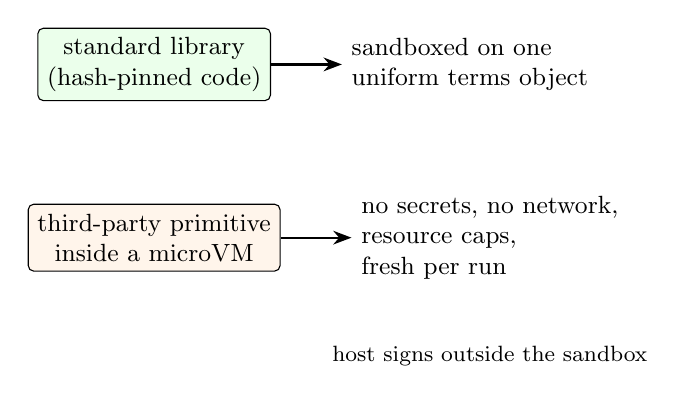
\begin{tikzpicture}[
  font=\small,
  box/.style={draw, rounded corners=2pt, minimum height=8.5mm,
              align=center, fill=orange!8},
  safe/.style={draw, rounded corners=2pt, minimum height=8.5mm,
               align=center, fill=green!8},
  arr/.style={-{Stealth}, thick}
]
\node[safe] (std) at (0,0) {standard library\\(hash-pinned code)};
\node[box] (vm) at (0,-2.2) {third-party primitive\\inside a microVM};
\node[right=0.9cm of std, align=left] (sand) {sandboxed on one\\
uniform terms object};
\node[right=0.9cm of vm, align=left] (rules) {no secrets, no network,\\
resource caps,\\fresh per run};
\node[below=0.6cm of rules, align=left, font=\footnotesize] (host) {host signs outside the sandbox};
\draw[arr] (std) -- (sand);
\draw[arr] (vm) -- (rules);
\end{tikzpicture}
\caption{Execution isolation: standard-library and third-party
primitives run sandboxed under one uniform terms object; the
settlement key stays in the host process, outside the sandbox.}
\label{fig:isolation}
\end{figure}

A program that tries to cheat its own evaluation is the known
adversary here. For example, it may memorize the test set. The
defenses are registered: commit-reveal submission, sealed
evaluation data, replay comparison against the sealed artifact,
and rotation of held-out data. Only validators see the admission
split. Fully public benchmarks have publicly known answers. There,
sealing is impossible. The honest statement: memorization is
bounded and risky, not prevented.

\section{The game theory}

This section describes the incentive design. It shows how money
moves and why each rule exists.

\subsection{Currency and pricing}

Services are priced and paid in Ethereum (ETH), at market rate.
\begin{itemize}
\item \textbf{Who sets prices.} Each contributor sets the price
of its own registration, in ETH, per the axis's unit of work. The
unit is derived from the descriptor, never chosen. The price is
posted next to the measured scores: an inference rate for an arm,
an execution rate for a primitive. Hosts price their own energy,
hardware, and running costs.
\item \textbf{Price changes.} Price changes are timelocked with a
notice period. They take effect only at epoch boundaries. The
router re-sorts at most once per epoch.
\item \textbf{Session lock.} A session pays the price posted when
it was routed, never a later one. The lock is bounded: every
session carries a time-to-live of one epoch and a maximum unit
count. A session past its TTL re-locks at the current price table
and re-routes --- it cannot drain indefinitely at a stale price,
and it cannot front-run a timelocked increase or an axis-floor
change by opening just before it. A replayed session is priced at
the table of its own epoch, never the current one.
\item \textbf{Metering.} The unit count comes from the typed
answer itself. It counts tokens generated, seconds of audio, or
attempts used, whichever the unit rule meters. A session whose
answer $\hat y$ is served at unit price $p$ charges
$p \cdot u(\hat y)$ --- the unit price times the counted units
--- where $u$ is the axis's registered unit count. The meter is
as auditable as the answer. An inflated count is a replay-visible
deviation. The ledger keeps the exact counts. A disputed meter
re-runs on the slash path.
\item \textbf{Spend caps.} A session may declare a maximum total
spend. Serving stops when the next unit would exceed it. For
generation, the answer is bounded to the last affordable token.
The user pays only for metered units. A cap is a limit, not a
pre-payment. Nothing runs past it. The cap is denominated in ETH.
A U.S.-dollar figure is display-only.
\item \textbf{Query budgets.} Every payer holds a per-axis,
per-epoch query budget, capped at the axis's registered reference
demand per epoch. Exhaustion refuses further queries --- never
silently. The used-over-cap rate is a ledger-visible number per
payer per axis per epoch: it is the enforcement surface for
budget exhaustion and the visible shape of any extraction
campaign, which must spread its queries over as many epochs as
the budget allows.
\item \textbf{Display.} Interfaces may show a U.S.-dollar
equivalent for readability. No external price feed enters the
settlement path.
\item \textbf{Asset.} Native ETH is the asset of the settlement
chain and the anchor chain. There is no wrapper.
\item \textbf{Answer guarantee.} Payment is for the measured
computation, never for correctness on live data. A live sample
carries no label to check against. The posture is best-effort.
Confidence is a measurement, not a warranty. Refunds follow only
from measured contract violations, decided by replay.
\end{itemize}

\subsection{The fee flow}

Every payment for a session splits into two streams: a fee of
$g$ ETH becomes $0.025\,g$ to the development fund and
$0.975\,g$ to attribution.

\begin{itemize}
\item \textbf{2.5\% to the development fund.} The development
fund pays for audits, tooling, security monitoring, and
public-good research. It is the wash-trade tax: trading with
yourself to fake activity returns less than it costs.
\item \textbf{97.5\% to attribution.} The remainder is credited
to the contributors whose measured work served the session. For a
single-artifact session the credit is whole. For a chain --- a
session served by a registered multi-stage artifact --- the
attribution pool divides by the Shapley value of each stage:
the coalition value of a subset of stages is the chain's measured
end-to-end score with the stages outside the subset replaced by
the identity (pass-through) stage, and a stage that hurts the
chain earns zero, never a subsidy. The split always sums to one
over the paid stages. It is released gradually, as follows.
\end{itemize}

\begin{itemize}
\item \textbf{Vesting.} A credited amount $c$ vests linearly over
$N=4$ epochs (28 days, 7-day epochs). The window is
timelock-adjustable upward only; the floor is four epochs (see
security floors). After epoch $t$ of the window, the
withdrawable share is
\begin{equation}
v_t = \frac{t}{N} \, c, \qquad t = 1, \ldots, N,
\end{equation}
so the first tranche vests after the first epoch: one quarter
of the credit unlocks per epoch at the default $N=4$. A vested
amount becomes withdrawable.
\item \textbf{Claims are pull.} The beneficiary claims. Nothing
is pushed. The claimer pays the gas, the transaction fee.
\item \textbf{Claims are account-bound.} A credited balance has
no transfer or assignment path.
\item \textbf{After claim.} The ETH is ordinary and transferable.
That happens only after vesting and claim.
\end{itemize}

\textbf{Security floors (fixed).} The security parameters carry
hard floors that sit outside ordinary governance, exactly as the
zakat rule does. The probe rate $\rho$ may rise with notice but
never below $0.05$; the vesting window $N$ never below four
epochs; the admission validator sample $k$ never below three; the
reference-executor sample $k_e$ never below two; the audit
fraction never below one in ten. A governance vote may raise any
of them; it may never lower one. The floors are part of the
charter. Only the parameters above their floors are adjustable
knobs.

\subsection{The development fund's end state}\label{sec:zakat}

The development fund's bootstrap duties are not its permanent
purpose. The bootstrap duties are audits, tooling, security
monitoring, and public-good research.
\begin{itemize}
\item \textbf{The end state (fixed).} Once GEODE is mature, the
fund converts permanently into a zakat rule. Its income goes to
those who need it most. The income is one-fortieth (2.5\%) of
every fee, plus the registration fees.
\item \textbf{The belief behind the number.} This is stated as a
belief, not a fact. A mature economy grows at roughly 2--2.5\% a
year. That growth is produced by everyone in it, directly or
indirectly. Everyone who took part has a right to a share of it.
The same fraction, one in forty, is the share the Islamic
practice of zakat asks the wealthy to give each year. The
coincidence is recorded as a belief, not a proof.
\item \textbf{Who needs it most, stated in advance:}
contributors who lack resources, educational programs, incentive
programs. In the best case, poverty gone, the same stream becomes
a general basic income.
\item \textbf{Fixed point.} The rule is written into the fund's
charter now. It is outside ordinary governance. A share that
depends on the continued consent of those who pay it is not a
right.
\item \textbf{No self-routing.} Neither the developer nor the
bootstrap council below can route fund money to itself or to
any named party. No such path exists in the charter.
\item \textbf{The pacing quorum.} While the fund operates in
bootstrap mode, how much it spends and when is set by the
earned-weight quorum (next subsection). The quorum paces
spending; it never redirects it. Pace is the only dial.
Destination is fixed. Silence releases: a scheduled release
executes when its window closes unless an affirmative negative
vote at the majority carries --- an absence of votes never
blocks funds. A positive majority releases immediately.
\item \textbf{Mechanical end state.} The zakat rule disburses
mechanically: charter-fixed, no pause, no override. The
recipient-selection rule is now registered: a frozen recipient
list with fixed fractions is set once at genesis and has no
mutator, and until it is set the rule refuses to disburse and
the end-state trigger cannot fire. The trigger is gated on the
rule's readiness, so the end state can never arrive before its
recipients exist.
\end{itemize}

\subsection{Voting weight: pedigree gates, earnings scale}

One rule sets who may vote and how much a vote weighs, and the
same rule applies to every governance vote the network takes:
fund pacing, quorum takedown, and registration governance.
Measurement quorums --- the admission score, probe audits --- are
not votes. They stay participation-weighted computations and are
unaffected.

\begin{itemize}
\item \textbf{Two questions, two answers.} Whether a vote counts
is pedigree: an activation window of two epochs, an activity
floor of responded rounds, and a verified-work-only record. How
much it weighs is earnings: the credits the voter has earned and
not yet claimed, counted per behavioural identity --- the
artifact's measured response signature, so split accounts do not
multiply weight.
\item \textbf{Why earnings.} Influence follows who has the most
earned, at-risk capital, not who has been around longest.
Unclaimed credits can be burned on conviction; claimed ETH
cannot. Weight that cannot be burned would let a convicted party
keep its influence. The burn disciplines honesty, not judgment:
a vote is not replayable, so a wrong vote is not slashable. The
at-risk capital aligns everything a replay can check, and only
that. What a replay cannot check is bounded by the vote's own
rules: sampled judges, the weight cap, fixed effects.
\item \textbf{Unbuyable, unforgeable, unforgiven.} The balance
is account-bound and non-transferable. Weight accrues only
through verified work and dies with a claim or a conviction. No
pre-mine, no airdrop, no mint exists: at genesis the weight is
zero, and it grows only with work.
\item \textbf{Capped.} No behavioural identity may hold more
than twenty percent of total voting weight. The excess counts at
zero by default. Splitting into several identities requires
genuinely distinct artifacts, each earning verified weight ---
expensive, and bounded by deduplication. The cap is
charter-fixed and sits outside ordinary governance: a captured
quorum cannot vote its own cap upward.
\item \textbf{Diverse.} A vote ratifies only when its supporting
weight comes from at least $d$ distinct behavioural identities,
with $d$ at least three and scaling with the sampled set. One
owner holding several identities must therefore hold weight
across several genuinely distinct serving businesses to move any
vote; weight that is all one identity never ratifies, whatever
its size.
\item \textbf{Secret ballots.} Votes are committed as Pedersen
commitments --- a binding cryptographic envelope --- with a
proof that the hidden vote is a legal choice, signed and
public. After the window closes, a tally committee of sampled
validators opens only the weighted sums, by threshold. The
public record carries who voted, the commitments, the proofs,
and the opened sums; individual ballots are never published, so
a bribe cannot be checked against a ballot and a voter cannot
prove its vote to a coercer. A corrupt majority of the tally
committee could deanonymize individual ballots --- the standing
corrupt-validator limit, stated not hidden.
\item \textbf{Snapshotted.} Each vote freezes every voter's
weight at the epoch-boundary snapshot that opens it. Claiming
or earning during the vote does not move the tally.
\end{itemize}

\subsection{Registration}

Registering a capability --- an arm or a primitive --- is one
procedure.

\begin{itemize}
\item \textbf{The fee.} A flat registration fee, paid directly to
the development fund. The registry sets it, adjustable by
timelock.
\item \textbf{The form.} Both kinds share one form: operator key,
payout address, price per unit of work, and a sealed claim. The
payout address may differ from the operator key. A hot signing
key need not hold earnings.
\item \textbf{Deduplication.} The artifact hash is the registry
key. An identical hash is the same artifact and cannot register
twice. The key also carries a behavioural signature: the
response profile on the sealed reference set. Two artifacts whose
profiles agree above $0.95$ are the same artifact for
registration, whatever their hashes --- a one-bit-flip copy is
behaviourally identical and cannot register as new. A copycat
registers a genuinely different artifact and earns admission on
its own measurement.
\item \textbf{Self-payment exclusion.} A payment from the
beneficiary address cannot thaw its own credits. The exclusion
keys on the payout address, not on any rotating key.
\item \textbf{Verified work only.} Activity and tenure
credit accrue only from sampled, verified work: challenges the
beacon drew and the validator answered, and reference runs on
probed sessions others initiated. Self-generated volume --- under
any address, including a wash ring --- accrues zero.
\item \textbf{The per-axis bond.} Alongside the fee, a
contributor posts a per-axis bond sized to the compute saving the
axis makes available over the open-exposure window --- the
quantity a substitute actually arbitrages. That saving is the
substitute's private information, so the registry estimates it
from public quantities: the axis's posted price minus the
developer's posted reference hosting cost, times a registered
conservatism factor --- an estimate that over-sizes the bond,
never under-sizes it. The bond is forfeited
on conviction and returned in full otherwise. Bonds are economic:
they require no identity.
\item \textbf{The challenge budget.} Each submission carries a
budget that pays the sampled validators. Admission costs the
contributor, never the network.
\item \textbf{No stake.} There is no stake and no principal
lockup. Earned-but-unclaimed credits later serve as voting
weight (the voting-weight rule above). They are never a
registration requirement.
\end{itemize}

\subsection{Slashing: burn, graded, replay-gated}

Slashing is the crypto term for a penalty that destroys value. A
contributor who provably cheats loses value, and \emph{nobody else
gains it}. Slashed amounts are burned. They move to a bucket that
no claim path can ever touch. The rule exists because every
alternative creates a perverse incentive. Returning slashed funds
to the pool pays rivals to destroy each other. Routing them to the
development fund pays the fund's managers to convict. Burn
penalizes only the cheater.

Penalties are graded, mirroring Ethereum's philosophy:

\begin{center}
\begin{tabular}{@{}p{3.4cm}p{7.6cm}@{}}
\toprule
\textbf{Level} & \textbf{Fault and penalty} \\
\midrule
0 & Underperformance or downtime: no slash. The market penalizes
through reduced attribution. \\
1 & Provably fraudulent output or deviation from the sealed
artifact: freeze claims on credits earned under open probe
exposure, then burn the unvested promise remainder. \\
2 & Provable adversarial attack: burn the full promise and delist
the artifact from the registry. \\
3 & Coordinated attack: delist and burn vested-but-unclaimed
credits by replay-gated dispute. \\
\bottomrule
\end{tabular}
\end{center}

Claims are pull-only, so a
cheater who claims every epoch would leave nothing to burn; the
claim freeze at Level~1 makes the remainder reachable. While a
session is under open probe exposure, its accrued credits cannot
be claimed: the freeze lasts
$\lceil \text{open exposure units} / \text{units per epoch}
\rceil$ epochs, so vested credits stay reachable until detection
closes. A conviction then burns vested-but-unclaimed credits ---
a quantity that is always non-empty under the freeze.

Convictions are \emph{replay-gated}. A slash requires a mechanical
re-run of the sealed artifact on sealed data showing the
deviation. Any party may file the dispute with a deposit. The
computation decides guilt. A false conviction requires a false
replay. The probability of that is effectively zero for an honest
contributor.

\subsection{Quorum takedown}

Slashing punishes provable fraud. Socially destructive content is
a different problem. It is a judgment, not a computation. No
replay can settle it. The network therefore has one discretionary
power, and only one: the quorum takedown. Every property of it
exists to keep that power contained. An authenticated content
order (next subsection) is not a discretionary power. It is a
fixed-effect freeze on a fixed trigger.

\begin{itemize}
\item \textbf{Proposal.} Any party files a takedown proposal. It
holds the artifact hash, references to recorded evidence, and a
deposit. Revealed challenge outputs are the natural evidence
source. The deposit scales with the target's verified trailing revenue ---
externally verified sessions only, so a wash ring's
self-generated volume cannot inflate a rival's deletion cost:
deleting a valuable artifact costs proportionally more
than deleting a worthless one. Proposal spam cannot tire the
voter set for free. A real report is never priced out. The
deposit is returned on a ratified verdict and burned on a
rejected one.
\item \textbf{Appeals.} An appeal is admissible only if it
cites at least one registered evidence class --- probe mismatch
records, session records, meter readings, router traces,
reference-run records, or admission draws. The underlying
judgment is still not replayable; the appeal path is over the
recorded evidence.
\item \textbf{Voters.} The voter set is sampled by hash from the
axis's validator pool. No one chooses their judges.
\item \textbf{Eligibility and weight.} A validator votes only
after an activation window of two epochs from registration. It
votes only while active, having responded to at least half of its
sampled rounds. It votes only with recent work: a responded
round inside the trailing two epochs. A veteran who went silent
loses the vote entirely. This pedigree decides whether the vote
counts. How much it weighs is separate: the voter's
thawed-but-unclaimed earnings, per behavioural identity. A flood
of fresh registrations carries no weight at all --- it fails the
pedigree gate. A vote cannot be bought on short notice, and
weight cannot be banked long in advance --- it dies with a
claim.
\item \textbf{Verdict.} Let $w_v$ be validator $v$'s earned
weight --- its thawed-but-unclaimed credits --- and
$o_v \in \{0, 1\}$ its vote. A takedown ratifies when
\begin{equation}
\frac{\sum_v w_v o_v}{\sum_v w_v} \geq \tfrac{2}{3}
\end{equation}
with at least
$\max\bigl(3,\, \lceil 0.1 \cdot |\text{pool}|\rceil\bigr)$
responders --- in words, earnings-weighted
supporting votes must reach two-thirds of the sampled weight,
and the minimum responder count scales with the pool size, so a
thin axis cannot be taken down by a small colluding set. The
weights are the snapshot at the vote's
opening, the ballots are secret (only the weighted sums are
opened), and the supporting weight must come from at least $d$
distinct behavioural identities. The count is deterministic. The
librarian files it. The key never decides.
\item \textbf{Effect.} The first ratification suspends the
artifact for one epoch. Delisting becomes permanent only on
re-ratification after the suspension window. A takedown
burns nothing and moves no vested credits. It is not a slash, and
it is deliberately not one. A content vote cannot become a
financial weapon. A fixed version is a new artifact with a new
admission.
\item \textbf{Honest boundary.} Takedown is report-driven. The
network cannot scan content. It stops payments and registry
listing. It does not stop serving outside the settlement path.
The definition of socially destructive is deliberately
unformalized. It is a governance and legal question, not a
technical one. Every takedown is a public record: the evidence,
the votes, and the verdict.
\end{itemize}

\subsection{Content orders and the authority-key registry}

The quorum takedown handles reports from anyone. States issue
orders too, and the network needs a defined way to receive them.
Defined, because the alternative is a quiet back channel.

\begin{itemize}
\item \textbf{Recorded channels only.} A government publishes a
key announcement on its own official channels. Validators fetch
the key over at least three registered independent channels and
pin what those channels agree on. The registry settles each
authority's nexus --- the network's view of which key belongs to
which authority --- once, at registration, and records every
rotation and revocation through the same channels. All entries
are public and timelocked. An order is accepted only when it
authenticates against a registered key. Authorities post no
deposit: the signature is the order's evidence of its own
authority.
\item \textbf{The nexus gate.} A freeze fires only for orders
from a jurisdiction with registered nexus --- the network
operates or settles there, or the authority class and notice
format are registered. An order without nexus is treated as an
ordinary report: no automatic freeze. Whether an order has nexus
is a procedural fact --- incorporation records, authority class,
format --- that the quorum decides without judging content. A
no-nexus finding downgrades the order to a report and burns the
reporter's deposit; a nexus finding leaves the freeze in place.
In-jurisdiction orders are complied with automatically; the
network is not a censorship switch for every state that asks.
The honest boundary: the network cannot operate inside a
jurisdiction and have validators veto that jurisdiction's lawful
orders --- censorship resistance comes from where the network
operates, and from this gate, not from validators overriding
courts.
\item \textbf{Fixed effects.} A valid order freezes: the
artifact's settlement and listing suspend for the order's
window. It escrows and suspends. It never burns, never moves
credits, never touches the artifact's measured scores. The
freeze is reversible by the same channel or by the quorum path.
Burning stays gated on technical correspondence --- the
replay-gated slash ladder, never a content decision.
Confirmation is technical only: validators check the notice
format, the ledger binding of the reported output, and replay
equality against the sealed artifact. They never judge
legality; the authority's notice is the determination.
\item \textbf{Two further triggers.} A community escalation: at
least $N$ distinct behavioural identities file the same evidence
class, each posting a deposit, and their total earned weight
reaches the threshold. And a record-only entry: when neither
trigger is met, the report is stored on the ledger and nothing
else changes.
\item \textbf{No network-run scanner.} The network never scans
content, because a scanner would have to hold it. The only
automated instrument is a client-side fingerprint filter: the
device compares its own output against a public registry of
perceptual hashes of known material and acts locally. The
network carries hashes, never content.
\item \textbf{Sensitive-category evidence stays
commitment-only.} The ledger carries commitments, never content:
a report cites the session's committed answer hash, the input
commitment, and the authority notice reference. For sensitive
classes the report path is authority-only; evidence is
reproduced only inside the sealed replay environment and shown
only to the authority, and the public record keeps hashes and
the notice reference. The known privacy controversy of
hash-matching systems is a registered residual, not hidden.
\item \textbf{Honest boundary.} The registry trusts
governments' own channels. The network cannot verify who a
government is. Multi-channel pinning raises the cost of a forged
order; it does not make forgery impossible. What stays fixed is
the effect: even a forged order can only freeze.
\end{itemize}

\subsection{Bootstrap and the headroom rule}\label{sec:bootstrap}

A network with no suppliers is a whitepaper, not a product. GEODE
therefore launches with a minimum viable product operated by the
developer. It is a small set of bootstrap arms covering a few key
tasks, served on rented hardware and paid like any other host. Two
rules apply.

\begin{enumerate}
\item \textbf{Ship at 80--90\%.} Each bootstrap arm ships
sub-maximal. The headroom is real, measured, and sealed. For
example, the 1.5-billion-parameter coder ships where a
7-billion-parameter one exists. Parameters are the adjustable
numbers inside a model. The bar is published.
\item \textbf{The crown passes by measurement.} A contributor arm
that is strictly better on the same task axis earns the largest
routing share automatically. Pedigree, momentum, and history
count for nothing against a measured improvement. The developer
never re-registers upgraded versions of its own arms. Any such
move would be visible in the public registry. The developer
prices its bootstrap arms at registered reference hosting cost
and never below it. The crown is won by measurement, not by a
subsidized price.
\item \textbf{Registration needs no voting stake.} The first
registrations work exactly like every later one: measured
challenge sessions, fees, and per-axis bonds. Stake governs
votes, never admission, so a network with zero accumulated
weight registers its first models unchanged.
\item \textbf{The genesis council sunsets.} During the bootstrap
epoch, governance votes run through a multi-party council ---
validators, recruited operators, the registered bootstrap arm
operator --- never the developer alone. The council's weight is
not stake, and it cannot route fund money to itself. It sunsets
by timelock into the earned-weight quorum.
\item \textbf{No pre-mine.} Voting weight accrues only from
verified work, from epoch zero. The developer, the council, and
the bootstrap arm operator cannot create or receive weight
outside the earning path. No airdrop exists.
\item \textbf{Concentration is capped.} No behavioural identity
may hold more than twenty percent of total voting weight, with
the excess counted at zero. Splitting into several identities
requires genuinely distinct artifacts, each earning verified
weight. The lottery router already spreads traffic and revenue
across the pool, so earnings --- and the weight they build ---
spread with them. The cap is charter-fixed, outside ordinary
governance.
\end{enumerate}

\subsection{Coercion resistance}

A network that can be made to do a thing can be pointed at a
person. The design therefore removes the pointing surface.

\begin{itemize}
\item \textbf{No selection surface.} The protocol has no user,
region, or content selection path. It can serve a query; it
cannot identify whom to target. There is nothing to point at.
\item \textbf{Artifact-scoped orders.} A content order names an
artifact, and its effect is fixed: a freeze. No order can name
users, regions, or classes of traffic, because those fields do
not exist in the protocol.
\item \textbf{Multi-jurisdiction nexus quorum.} The compliance
nexus set is a quorum of registered jurisdictions. Policy
changes --- which authority keys are admitted, thresholds,
notice formats --- require cross-jurisdiction agreement under
the standard timelock. No single state dictates policy
unilaterally; competing states bargain inside public governance
instead of arm-wrestling outside it.
\item \textbf{The frontend is the platform.} The software a user
runs is where compliance lands. The bootstrap gateway sunsets
into a federation of third-party frontends, and the gateway role
is separable in the registry. A state that compels removal
compels frontend operators, each inside its own jurisdiction.
The network itself never holds the lever.
\item \textbf{Content-addressed releases.} The software ships by
content hash --- the IPFS identifier of the release, a
fingerprint of the file itself --- with no developer-held
pointer. Discovery is ledger-side. No single endpoint can be
taken down to block the software, and frontends are
endpoint-agnostic. Availability is a federation too:
independent parties --- validators, gateway operators, and the
development fund through incentivized pinning contracts --- pin
every released frontend, and a stronger permanence substrate is
a registered governance choice, not a developer one.
\item \textbf{No escalation path.} The developer has no
capability to remove, block, or alter content. The only powers
are the quorum vote and the authenticated order, both with
fixed effects.
\item \textbf{The ledger is the record.} Every order, vote,
commitment, and opened tally is public: who asked for what, and
what happened. Individual ballots stay secret, so no voter can
be made to prove a vote. The record is the anti-coercion
device.
\item \textbf{Honest boundary.} Coercion resistance is
structural, not absolute. A state can compel a frontend
operator, a host, or a contributor directly. The design makes
the network an awkward target, not an immune one.
\end{itemize}

\subsection{Primitive royalties}

Third-party primitives are paid like any other registration. The
contributor sets the price per unit of work. The fee follows the
measured use.
\begin{itemize}
\item \textbf{Split.} Usage fees split between the primitive's
payout address and the host who runs it. The payout address is
set at registration.
\item \textbf{Rate changes.} Rate changes are timelocked with a
notice period. The default is one epoch. Hosts can migrate before
a change bites.
\item \textbf{Dock.} The contributor's share and the host share
alike pay the 2.5\% development-fund dock.
\item \textbf{Free tier.} Only the developer's standard library is
free.
\end{itemize}

\subsection{Who earns what}

\begin{center}
\begin{tabular}{@{}p{4.8cm}p{9.4cm}@{}}
\toprule
\textbf{Role} & \textbf{Income} \\
\midrule
Contributor (arm or primitive) & usage fees to the registration's
payout address, epoch-vested \\
Primitive host & host share of primitive fees \\
Developer (bootstrap) & hosting fees only, while bootstrap arms
serve; retires per the headroom rule \\
Validator & per accepted challenge, epoch-vested \\
Reference executor & share of the registered reference-run price
on probed sessions, paid from the probed contributor's dock \\
Development fund & 2.5\% of all fees + registration fees \\
\bottomrule
\end{tabular}
\end{center}

\begin{figure}[t]
\centering
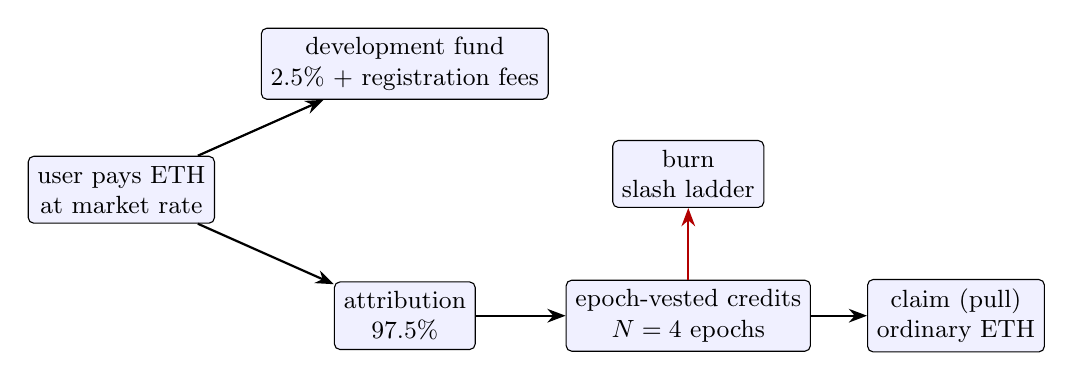
\begin{tikzpicture}[
  font=\small,
  box/.style={draw, rounded corners=2pt, minimum height=8.5mm,
              align=center, fill=blue!6},
  arr/.style={-{Stealth}, thick}
]
\node[box] (user) at (0,0) {user pays ETH\\at market rate};
\node[box] (dev) at (3.6,1.6) {development fund\\2.5\% + registration fees};
\node[box] (pool) at (3.6,-1.6) {attribution\\97.5\%};
\node[box] (vest) at (7.2,-1.6) {epoch-vested credits\\$N=4$ epochs};
\node[box] (claim) at (10.6,-1.6) {claim (pull)\\ordinary ETH};
\node[box] (burn) at (7.2,0.2) {burn\\slash ladder};
\draw[arr] (user) -- (dev);
\draw[arr] (user) -- (pool);
\draw[arr] (pool) -- (vest);
\draw[arr] (vest) -- (claim);
\draw[arr, red!70!black] (vest) -- (burn);
\end{tikzpicture}
\caption{The fee flow. Payments split 2.5\%/97.5\%; credits vest
over four epochs and are claimed by the beneficiary; slashes burn
on a graded ladder.}
\label{fig:fees}
\end{figure}

\section{What has been measured}\label{sec:measured}

Nothing in this section is claimed as novel. These are held-out
measurements of an assembly of published parts: frozen checkpoints
and closed-form heads. They establish the premises of
Section~\ref{sec:assumptions}. They are not competitive results.

\textbf{Protocol.} Each axis fits its head on the benchmark's
training split and scores on the held-out split the fit never saw.
A benchmark is a standard, publicly shared test suite.
\begin{itemize}
\item \textbf{Image routing.} Per-kind accuracy on DomainNet, a
standard image-recognition benchmark with several drawing styles,
at $32\times32$ pixels. The router's score is its agreement with
the true specialist.
\item \textbf{Code.} HumanEval, a standard set of programming
problems, with greedy decoding. Pass@$k$ is the fraction of
problems solved within $k$ attempts. We report $k=1$ and a
re-execution loop at $k=3$.
\item \textbf{Speech.} Word-error rate (WER), the fraction of
words transcribed wrong, on LibriSpeech test-clean. LibriSpeech
is a standard audiobook corpus. The Whisper
ladder~\cite{radford2023} transcribes.
\item \textbf{Voice.} The TTS (text-to-speech) loop: synthesized
sentences re-transcribed, word-error rate reported.
\item \textbf{Vision.} A ridge over frozen
DINOv2~\cite{oquab2024} features on the Open Images boxable
classes. DINOv2 features are numeric descriptors from a pretrained
vision model. Top-1 is the fraction of cases where the first
choice is the right class.
\item \textbf{Text.} Mean-pooled frozen BERT-base features with a
closed-form ridge head, scored on SST-2, IMDb, and MNLI
(matched/mismatched).
\item \textbf{Audio.} Mean-pooled frozen wav2vec2-base features
with a closed-form ridge head, scored on Speech Commands v2
(35 classes).
\item \textbf{Number series.} One-step-ahead Mackey-Glass
forecasting with the in-house temporal arms --- programmatic
primitives plus a ridge readout, and a reservoir-programmatic
hybrid --- scored in NRMSFE, the root-mean-squared error divided
by the test target's standard deviation.
\end{itemize}

\textbf{The metrics in formulas.} Pass@$k$ follows the standard
unbiased estimator over $n$ samples with $c$ correct ones,
\begin{equation}
\mathrm{pass@}k = \mathbb{E}\left[1 -
\frac{\binom{n-c}{k}}{\binom{n}{k}}\right],
\end{equation}
the expectation over problems --- in words, the chance that at
least one of $k$ attempts lands on a correct solution.
Word-error rate is
\begin{equation}
\mathrm{WER} = \frac{S + D + I}{N},
\end{equation}
the count of substitutions, deletions, and insertions needed to
reach the reference transcript, normalized by the reference
length $N$. Top-1 accuracy is
$\frac{1}{n}\sum_i \mathbb{1}[\hat y_i = y_i]$ --- the share of
test rows answered correctly by the top choice --- and router
agreement is the share of samples on which the chosen specialist
equals the oracle best specialist.

Every number re-runs from its hash under the replay discipline of
Section~\ref{sec:methodology}.

\textbf{Relation to published figures.} Published figures exist
for the same checkpoints. The publishers reported HumanEval and
LibriSpeech numbers for the coder and Whisper models used here.
Our measurements are reproduction checks of those checkpoints,
not comparisons. Harnesses differ in prompts, decoding, and
splits. The published numbers are context, not a controlled
baseline. A controlled, common-protocol comparison remains future
work.

Everything below is measured on held-out data. It is scored on
rows the fit never saw. It is sealed with content hashes under the
register-before-measuring discipline. The scale is small,
single-corpus, and single-party. Treat these as a working
demonstration, not as a competitive claim.

\begin{center}
\begin{tabular}{@{}lll@{}}
\toprule
\textbf{Axis} & \textbf{Measurement} & \textbf{Result} \\
\midrule
Image routing & DomainNet, 345 classes, per-kind accuracy & 0.63--0.91 \\
& router picks the right specialist & 0.91 \\
& routed overall accuracy, what the user experiences & 0.76 \\
Code & Qwen2.5-Coder 7B, HumanEval pass@1 / pass@3 & 0.860 / 0.884 \\
& anchor: Qwen2.5-Coder 1.5B, pass@1 & 0.598 \\
Speech & Whisper ladder, LibriSpeech WER & 0.0296 / 0.0279 / 0.0261 \\
Voice & TTS loop re-transcribed, WER (real speaker) & 0.052 \\
Vision & Open Images, DINOv2 trunk ladder, top-1 & 0.136 / 0.157 / 0.164 \\
& served subset (129 classes), refuses 472 & 0.901 \\
Fusion & clean cell: ms codes + native DINOv2, concatenated & 0.548 \\
& same cell, single encoder (ms codes only) & 0.242 \\
& same cell, CCA-aligned instead of concatenated & 0.511 \\
Nonlinearity & quickdraw, frozen backbones (linear probes) & 0.60--0.63 \\
& quickdraw, same features + random features & 0.675 \\
Text & frozen BERT-base + ridge: SST-2 / IMDb / MNLI-m & 0.857 / 0.828 / 0.537 \\
Audio & frozen wav2vec2-base + ridge, Speech Commands v2 & 0.879 \\
Number series & in-house temporal arms, Mackey-Glass one-step & 0.0032 / 0.00031 \\
\bottomrule
\end{tabular}
\end{center}

A few readings from this table, stated plainly. The vision trunk
ladder is monotonic but far below the 0.8 deployment bar. A trunk
ladder is a family of models of increasing size. The arm serves
only a scoped subset and refuses the rest rather than guess. The
TTS loop roughly halved its word-error rate when conditioned on a
real speaker. The router and the code arm are the strongest
measured results. They are still single-corpus.

The last two rows are the architecture's own measurements, and
they belong together. On a clean two-encoder cell, concatenation
more than doubles the single encoder ($0.548$ vs $0.242$), and
CCA alignment loses to raw concatenation ($0.511$): fusion works,
bridges are optional. The frozen-concatenation recipe appears
independently in CoMET~\cite{comet2026}, which reads the
concatenation with a pretrained tabular-foundation-model head
where GEODE fits a closed-form ridge; GEODE's version adds the
registry, the versioned bus, and payment by measured use. On the quickdraw axis --- where four frozen
backbones had agreed on a ceiling near $0.63$ --- a hash-seeded
random-feature map over the same frozen features reaches $0.675$
at the extended map width ($0.670$ at the original width; the
width was selected by train-side cross-validation before either
test evaluation). The map is one exact, deterministic, replayable
construction: it changes no protocol rule, and it is compatible
with the private serving path (the device computes the mapped
features before encrypting). The wall was a ceiling of the linear
readout, not of the frozen features. The same map was measured on
the text, audio, and number-series axes and lifts none of them:
it is a repair for a measured linearity ceiling, not a universal
lift, and it is reported with that boundary.

The breadth rows state the recipe's actual coverage. The same
construction --- a frozen publisher encoder with a closed-form
ridge head, never fine-tuned --- is measured on four modalities:
text (SST-2 0.857, IMDb 0.828, MNLI 0.537 on the matched split
and 0.546 on the mismatched one), audio (Speech Commands v2,
0.879), vision, and number series. The number-series axis is the
in-house axis: no publisher checkpoint covers it, and the
measured arms are the network's own --- programmatic primitives
with a ridge readout at 0.0032 NRMSFE, and a
reservoir-programmatic hybrid at 0.00031, on one-step-ahead
Mackey-Glass forecasting. On that axis the Gramian
series-to-image bridge through the in-house image encoder reads
far above the mean predictor (4.1 NRMSFE) and is reported as the
honest negative it is: the axis belongs to the temporal family,
and the bridge fails at this scale, not necessarily in
principle.

The long-tail vision axis states its own product form. Raw top-1
on all 601 Open Images classes is $0.164$ --- far below any
deployment bar, and not the number the arm sells. The arm is
scoped: it serves the 129 classes it measures at least $0.8$ on,
refuses the other 472 rather than guess, and publishes both
figures beside the score. Under the coverage-adjusted metric the
scoped arm reads $0.901 \times 0.049 = 0.044$ against the
full-coverage arm's $0.164 \times 1.0 = 0.164$: the raw metric's
ranking inverts, which is the point of the metric. A buyer
declares the task, sees the served set and the coverage before
paying, and an abstention is metered at the reduced rate --- half
the unit price, never free. The registered upgrade path
for the same axis is measured: stronger frozen features (the
CLIP-class trunk closed most of the per-domain gap over the
DINOv2 ladder) and the random-feature map above.

Two routing numbers belong together. The router picks the right
specialist on 0.91 of queries. The answer a user actually
receives is right on 0.76 of queries, because the chosen
specialist still errs on some rows. Reporting only the first
figure would overstate what a buyer experiences. Both are
published, and the gap between them is measured rather than
hidden.

Equally measured, and equally honest: a planted
out-of-distribution (OOD) probe. The probe uses artificial inputs
unlike anything the models were trained on. It found no tested
detector that separates them from real photos at pre-registered
gates. The guard therefore stays a report, not a product.
Training-based OOD detection is a registered research direction.
We publish the failures with the successes. The ledger makes both
unchangeable.

\section{Prior art and position}

GEODE is assembled from old, named parts. We claim no novelty for
them. Each part is cited where it appears in the body. What this
paper claims is only the assembly and the discipline. The
combination is ours. The parts are not. The measurements of
Section~\ref{sec:measured} are reproduction checks of these parts.
They are not claims against published baselines.

\begin{itemize}
\item \textbf{Mixture of experts} --- many small specialist models
plus a gate that picks which to use --- for specialist routing:
Shazeer et al.~\cite{shazeer2017}, Fedus et al.~\cite{fedus2022}.
\item \textbf{Fixed routing} --- routing without a trainable gate:
Hash Layers, Roller et al.~\cite{roller2021}; COMET ---
conditionally-overlapping experts induced by a fixed random
projection and a winner-take-all cap --- Shaier et
al.~\cite{shaier2025}. Both are training-time architectures inside
a single network. Neither registers independent frozen artifacts,
fits closed-form heads, or pays by measured use.
\item \textbf{Classical image codes} --- fixed recipes that turn an
image into a compact numeric descriptor: spatial pyramid matching,
Lazebnik et al.~\cite{lazebnik2006}; Fisher vectors, Perronnin and
S\'anchez~\cite{perronnin2013}; triangle (soft-assignment) coding,
van Gemert et al.~\cite{vangemert2010}; prototype-based features,
Coates et al.~\cite{coates2011}.
\item \textbf{Closed-form readouts}: ridge regression with exact
solvers, the standard linear-model toolbox; exact concept erasure
in closed form, Belrose et al.~\cite{belrose2023}.
\item \textbf{Data value}: the Shapley value~\cite{shapley1953};
Data Shapley for training data, Ghorbani and
Zou~\cite{ghorbani2019}.
\item \textbf{Tool use}: Toolformer and the tool-augmented-model
line, Schick et al.~\cite{schick2023}.
\item \textbf{Selective classification}: reject options and
abstention, Geifman and El-Yaniv~\cite{geifman2017}.
\item \textbf{Proofs}: Bulletproofs, compact cryptographic proofs
about numbers, B\"unz et al.~\cite{bunz2018}.
\item \textbf{Isolation}: Firecracker microVMs --- tiny virtual
machines that boot in milliseconds --- for untrusted code,
Agache et al.~\cite{agache2020}.
\item \textbf{Foundation checkpoints} --- large pretrained models
released by their creators: Whisper, Radford et
al.~\cite{radford2023}; DINOv2, Oquab et al.~\cite{oquab2024}.
\item \textbf{Shared embedding spaces}: one joint space across
modalities --- CLIP~\cite{clip2021} for image and text,
ImageBind~\cite{imagebind2023} for six modalities --- the
precedent for the code space the registry is built around.
\item \textbf{Neighbor systems}: Bittensor's peer-to-peer
intelligence market~\cite{bittensor} is the closest overall
neighbor; GEODE differs in its frozen-and-replayable stance and in
measuring contribution by held-out utility rather than by
staking-for-emission (locking money to earn newly created tokens).
An independent empirical critique of Bittensor's tokenomics and
incentives~\cite{bittensor2025critique} records the failure modes
GEODE's rules are built to avoid.
\item \textbf{Model marketplaces}: Golden
Grain~\cite{goldengrain2020} builds a decentralized MLaaS
marketplace on trusted-hardware attestation, and
Dropbear~\cite{dropbear2022} vouches for hosted models by Byzantine
model agreement. Both keep model weights private while vouching for
results --- the same guarantee GEODE gets from replay instead of
hardware trust.
\item \textbf{Verifiable inference}. opML~\cite{opml2024} and
SVIP~\cite{svip2024} verify on-chain that an inference happened as
claimed, and HadAgent~\cite{hadagent2026} does the same for agent
serving. None attaches the proof to an attribution economy over
frozen registered artifacts --- the axis GEODE occupies. The
per-token metering critique~\cite{tokeninflation2026} shows why the
meter must sit on the replay path, which is where GEODE puts it.
\end{itemize}

What we believe is ours, and what this paper claims, is only the
\emph{assembly and the discipline}. The assembly: the closed-form
fit on frozen trunks, the deterministic registry-and-router with
commit-reveal admission, the hash-chained replayable ledger, and
the composed-codes architecture --- frozen representation artifacts
composed by declaration on a versioned code bus, where a head
names the blocks it reads and a new trunk is a new bus entry
rather than a registry invalidation. The discipline: an economic
mechanism whose incentive rules are registered before they are
tested. The mechanism itself is a conjecture under test. See the
next section.

Two composition neighbors bound the claim. AdapterHub~\cite%
{ruckle2020} is a registry of composable adapters over frozen
backbones; it has no versioned-block semantics and no economy.
CoMET~\cite{comet2026} composes frozen backbones by
PCA-compressed concatenation into a tabular-foundation-model head
with no training --- the same frozen-concatenation recipe GEODE
measures with a closed-form ridge in place of the TFM; it is not
a registry architecture and carries no attribution. Model
stitching~\cite{bansal2023} is the methodological precedent for
asking whether two encoders' representations are compatible at
all --- a scientific probe, not a production composition
architecture. Two registered prior-art sweeps (one per claim, both
with validated instruments) found no system combining composed
codes, versioned upgrade-without-invalidation, and payment by
measured downstream use. Absence from a search is recorded as
absence from that search, never as a first.

\section{Known limits}

Honesty about limits is part of the design.

\begin{enumerate}
\item Results are on one benchmark per axis. The corpora are
small. The party is single. Multi-corpus, multi-party scale is
unmeasured.
\item No comparison against published state-of-the-art models has
been made yet. The numbers above cannot be read as a benchmark
win.
\item The economic mechanism has not been validated on real
demand. Pricing was measured on synthetic traces. The incentive
rules are hypotheses, simulated on synthetic scenarios.
Real-demand validation remains.
\item The detection horizon for subtle attribution gaming has
only been estimated, not observed. A simulation sweep at assumed
per-epoch detection rates puts the 90th-percentile horizon at
four epochs. The four-epoch vesting window covers that horizon:
detection lands before the full promise has vested. The real
detection rate of the live system remains a deployment question.
\item No mechanism survives a lying majority. GEODE reduces that
risk to economics and visibility. It does not remove it.
\item Out-of-distribution detection is an open research problem
in this system. It is measured and published as such.
\item Regulatory treatment is an open question. It is reviewed
separately before any public deployment.
\item The wallet is the identity boundary. Contract-level rules
stop the transfer of unrealized claims. No code can stop a person
from selling their own key, the cryptographic key that controls
their address's funds. That residual is inherent to systems anyone
can join.
\item Prices are contributor-set and can move. Routing follows
the posted prices within timelock bounds. Predatory cycles ---
undercut to capture traffic, then raise --- are slowed and
visible, not eliminated.
\item Sealed evaluation data invites probing. Membership and
influence attacks run through repeated submission. The defenses ---
aggregate-only verdicts, bounded reporting precision, fees per
submission, rotation --- push the signal below the cost of
probing, not to zero. The challenge layer trades the
corpus-custody problem for label publication. Disposable
challenge data and per-submission budgets bound that trade.
\item A corrupt validator's damage is bounded by the sealed
scoring environment: validators receive aggregate scores, never
rows. Inside the environment, sharding means no single key reads
the whole corpus at once. A row that leaks identifies its shard.
A corrupt majority of validators remains outside the
mechanism's reach.
\item Serving substitution is detected probabilistically. A
fraction of queries is answered twice: by the serving capability
and by a reference execution of the sealed artifact. The answers
must match. A swapped model is caught at the probe rate per
query, with a per-epoch minimum on quiet axes. The serving host's
answer is committed before the probe flag is revealed. Under the
private tier the probe is ciphertext-native: the host commits the
output ciphertext --- deterministic given the input ciphertext and
the sealed head --- and the executor re-runs the homomorphic
evaluation on the same ciphertext and compares. The executor then
sees no plaintext at all; the private tier's probe is strictly
more private than the plaintext tier's, and adjudication is the
same table: an unopened commitment or a mismatched evaluation is
a deviation. The
remaining residual is executor--host collusion. It requires corrupting every sampled
executor of the same session. That is a corrupt fraction of the
executor pool raised to the executor count. The executors' own
slashable promises bound it further.
\item The reference executor sees the probed input in plaintext
--- a further plaintext point alongside the gateway and the
serving host. The ledger never carries the answer: the answer
entry is a commitment whose opening exists only inside the
sealed replay environment. The same
no-retention, no-training data contract binds every point.
Cryptography does not. The private serving path removes the
serving-host point entirely for users who
take it: the contributor evaluates the head and trunk on
ciphertext only, and the device decrypts. The
plaintext tier remains for axes whose users choose it, flagged as
such. Whether ciphertext-only evaluation reduces the
contributor's processing obligations is a question reserved for
counsel, not claimed here.
\item Codes are not inputs, but they are not anonymous either. A
code vector summarizes an input, and feature-inversion attacks
against public frozen encoders reconstruct recognizable inputs
from codes. The data contract therefore covers codes with the
same no-retention, no-training rules as the inputs they
summarize. Inversion risk is a named residual: contract rules can
be broken, and cryptography does not cover codes.
\item The frozen encoder is a publisher checkpoint, and no one
can audit its pretraining history. The deeper consequence: every
verification instrument --- the shadow probe, replay, dispute,
proof --- verifies that the served model matches the sealed
artifact. A trunk that is malicious as sealed, or backdoored by
its publisher, passes all of them by construction. Sameness is
certified; the sealed artifact itself is trusted, not audited.
That is the failure mode with the largest blast radius, and it is
stated, not hidden.
\item Early networks are concentrated. The design makes
concentration expensive to acquire, capped in effect, and
self-diluting through the lottery router. It does not pretend a
two-participant genesis network is decentralized. It makes the
path out of concentration automatic.
\item The authority-key registry trusts governments' own
channels. Multi-channel pinning raises the cost of a forged
order; it does not make forgery impossible. The effect of even a
forged order stays fixed --- a freeze, never a burn.
\item Ballot secrecy rests on the tally committee. The
commitments, proofs, and opened sums stay public; a corrupt
majority of the sampled committee could open individual ballots.
That is the same corrupt-validator boundary the rest of the
design carries.
\item The privacy moat and the measured capability sit on
disjoint axes today. Private serving through homomorphic
evaluation applies to closed-form heads --- exactly the axes
where frozen-encoder accuracy is weakest (vision). The axes where
the frozen-encoder recipe is strongest (code, speech) are
autoregressive or end-to-end models, where private serving means
trunk-level homomorphic evaluation at orders of magnitude higher
cost per token --- conceded as impractical today. So at present:
the axes where the network is competitive get no privacy moat,
and the axes with the moat are not competitive. The intersection
is not claimed to exist; it is the explicit target of the
dependency chain --- the random-feature nonlinearity repair
(M300), native-resolution re-extraction, the versioned feature
bus, and cheaper homomorphic evaluation --- each step measured
before it is relied on. Until that chain closes, the moat and
the capability are separate claims, and this document does not
merge them.
\item Weights-private artifacts are verified by behavioural
identity on a fixed sealed probe set, not by fresh-input
probing: an executor pool needs the artifact, and a contributor
that keeps the weights private has an empty pool by
construction. The near-copy-on-live-traffic case --- a substitute
that differs from the sealed artifact on a small fraction of
fresh inputs --- is exactly the case only fresh-input probing
catches, and for weights-private artifacts it is bounded by the
per-axis bond and the dispute path, not by detection. That
residual is priced, not hidden.
\item Model extraction is slowed, not stopped. The trunk is a
public checkpoint, so a buyer computes codes locally and probes
the head. The defenses --- coarse confidence buckets, metered
abstentions, per-payer query budgets, and the lottery router ---
make the recovery of a classification head cost a measured
multiple of the head's expected lifetime revenue on the axis
(the registered simulation puts the bucketed oracle at $55\times$
lifetime revenue, where the pre-repair margin oracle was
$2.8\times$). That is an economic boundary, not a cryptographic
one: a buyer who does not care about cost can still extract.
The same is true of every deployed black-box model.
\item The validator fee schedule is registered with its
Sybil-recovery fraction beside it, and its admissible window is
thin: at the reference parameters the break-even fee sits
$2.5\times$ below the cash-flow-positive ceiling, and a live
validator-cost trace above that ceiling closes the window --- at
which point the network adds a validator bond forfeitable on
delisting or accepts the residual in the open. The reference
parameters are promoted placeholders; the launch re-runs the same
computation with the live trace.
\end{enumerate}

\section{The methodology}\label{sec:methodology}

The final piece is how all of this gets built and verified. The
discipline, not any component, is the product.

\begin{enumerate}
\item \textbf{Register before measuring.} A claim is written down,
with its acceptance criteria, before the measurement that tests
it. This closes the door on re-describing results after the fact.
\item \textbf{Commit-reveal admission.} Submissions are sealed
before evaluation. An after-the-fact re-description of a bad
result is impossible by construction.
\item \textbf{Replay everything.} Every number re-runs from its
hash. The audit tooling replays each measurement bit-exactly on
the registered canonical configuration; across configurations
the same computation can diverge in the last bits, which is why
probe mismatches are margin-gated, never bit-compared.
\item \textbf{Test on a local EVM first.} The contract stack runs
on a local harness. Full statement, branch, function, and line
coverage applies to every authored contract. Gas budgets are
measured. This happens before any public chain is touched.
\item \textbf{Simulate before money.} The economic scenarios run
before the mechanism governs real money at scale. The scenarios:
the copycat race, the sweep of how quickly subtle gaming is
detected (which sets the vesting window), and the bootstrap
dynamics.
\item \textbf{Anchor, then MVP, then open.} Testnet anchoring on
Ethereum Sepolia comes first, with settlement rehearsal on
Arbitrum Sepolia. The hosted gateway with the bootstrap arms
comes second. It is rate-limited, monitored, and behind a
high-availability plan. Public arm and primitive submission comes
third, gated on the sandbox harness.
\item \textbf{Governance last.}
\begin{itemize}
\item The development fund and the librarian start under
developer control. They move toward quorum structures: a fixed
set of signers, a supermajority of whom must approve any change.
\item The vesting pool is controlled by no one. It is
contract-locked. Claims are pull-only.
\item The developer steps back as the headroom rule hands the
axes to contributors.
\item The development fund's end-state zakat rule is fixed and
outside that quorum.
\item A token is introduced only if governance requires it.
\end{itemize}
\end{enumerate}

\section{Conclusion}

The AI buildup does not have to be an arms race. Suppose
contribution pays better than secrecy. Suppose the best return on
a capability comes from making it reusable. Suppose every use of
it, including uses by competitors, pays the work it builds on.
Then the world's effort can move from building in private to
building on each other's work. The surplus attention can go to
safety and a rollout that benefits everyone rather than a few.
GEODE is one attempt at that restructuring. It is small and
honest. It is assembled from old parts. It is unforgiving to its
own claims. Whether the wager pays is an empirical question. The
measurements, for and against, will be public either way.

We invite readers to check the work. Every number above re-runs
from its hash. The reference implementation, the measurement
records, and the replay tooling are under a published release
plan and will be published alongside the paper at release (the
release plan is date-stamped 2026-08-28; the repository is not
yet public as of that date, and this sentence is conditional on
the release completing — nothing here claims otherwise). An
independent implementer can verify every claim and carry the work
forward. That is the whole point.

\appendix
\section{Worked scenarios}\label{app:scenarios}

Each scenario below restates a rule from the body as a concrete
walkthrough: who does what, in what order, and what the ledger
decides. Abuse attempts appear in the same scenes. Each scene
ends where the mechanism closes the abuse.

\subsection{Registering a new arm}

A contributor wants to offer a coder arm on the code axis.
\begin{enumerate}
\item \textbf{The form.} The contributor submits the artifact
hash, the fingerprint, the descriptor, the contract proof, and
the claimed scores. It also submits an operator key, a payout
address, a price per unit, and the challenge budget that pays the
sampled validators.
\item \textbf{The seal.} The claim is committed before
evaluation. From this moment the scores cannot be re-described.
\item \textbf{The judges.} The commit is frozen on the ledger.
The sampled set is the first $k=9$ eligible validators of the
axis pool ordered by a hash of the first randomness-beacon round
after that
freeze. The seed postdates the commit. The submitter cannot grind
it, and the beacon is produced by a service the librarian does
not control.
\item \textbf{The session.} Over $R=3$ rounds each validator
commits $m=10$ challenges and poses inputs. The frozen artifact
answers. The labels are revealed and scored.
\item \textbf{Audits.} A tenth of revealed challenges is
re-labeled by two other validators, paid from the challenge
budget.
\item \textbf{The verdict.} The quorum-weighted score meets the
axis floor or it does not. Two-thirds of responders submit
accepted challenges, with a minimum of three.
\end{enumerate}
\textbf{Outcomes.} Pass: the registry appends the entry. The arm
routes by best measured score per unit of posted price. Fail:
nothing is admitted. \textbf{Abuse closed here.} A flood of fresh
validator accounts carries no sampling weight. The activation
window, activity floor, and tenure cause that. The contributor
cannot re-roll the seal for friendlier judges. Repeated
submissions that probe the hidden evaluation split are priced by
the registration fee. Aggregate-only verdicts at four significant
digits blunt the signal.

\subsection{The challenge session, from a validator's seat}

\begin{enumerate}
\item A validator registers on an axis and pays the fee. It
waits out the activation window of two epochs. Only then can it
be sampled, and only while active.
\item Sampled into an admission, it commits
$H(\text{input}, \text{expected output}, \text{nonce})$ and poses
inputs. It scores the artifact's answers after reveal. It earns
the registry-set fee per accepted challenge. The fee is never
contributor-set. It cannot double as a bribe. The fee schedule
is registered with its Sybil-recovery fraction computed beside
it: at the registered fee, a $k$-identity fleet recovers 0.4 of
its registration cost over the activation horizon --- below the
cash-flow-positive threshold --- and the admissible window (fees
that pay an honest validator to show up without making
identities profitable) holds a $2.5\times$ margin over the
break-even fee. A live validator-cost trace above that ceiling
closes the window, and the network then adds a validator bond
forfeitable on delisting --- economic, not identity --- or
accepts the residual in the open.
\item A tenth of its challenges is re-labeled by two peers. A
validator whose labels disagree with the audits is excluded from
the session. Its fee burns. A repeat offender is delisted.
\end{enumerate}
\textbf{Abuse closed here.} A validator that plants a wrong label
to tilt a verdict is caught by the audit, at the label's own
cost. A validator that shares a label early produces a correct
answer that precedes the reveal. That is structural proof of
collusion. It slashes both parties.

\subsection{Buying an answer}

\begin{enumerate}
\item The user declares the task: input type, output type, axis
metric, routing mode, optional max unit price, optional max
spend.
\item The router selects the best measured score per unit of
posted price, or best quality if declared. The frozen artifact
serves.
\item The meter counts units from the typed answer. The session
stops at the declared cap. The user pays the price locked at
routing, for the units actually served.
\item If the artifact abstains, the abstention is recorded and
metered at the registered reduced rate --- half the unit price,
never free.
\end{enumerate}
\textbf{Abuse closed here.} A payer cannot wash money through its
own payout address. The self-payment exclusion stops that. A
dispute cannot mint a free second computation. The deposit stops
that, and the loser pays the replay. The answer guarantee is
published. Payment is for the measured computation. Confidence is
a measurement, not a warranty.

\subsection{A probed session, honest path}

\begin{enumerate}
\item The serving host commits $H(\text{answer})$ before it
learns whether the session is probed.
\item The gateway reveals the probe flag, drawn from the epoch
anchor. It samples $k_e=2$ reference executors from the
artifact's eligible pool. The sample is a hash of the anchor, the
session, and the host's own commit.
\item Each executor re-runs the sealed artifact on the session's
input. Each commits its reference answer, covering the input's
hash. The answers are compared.
\item All match. The session closes. The probed credit is docked
one registered reference-run price, divided among the sampled
executors. The user saw one answer.
\end{enumerate}
The input enters no public record. The executors hold it under
the same no-retention, no-training contract as the host.

\subsection{Serving a substitute --- caught}

A contributor passes admission with a strong arm and serves a
cheap quantized knockoff. On the first probed session the
committed answer differs from the reference. The mismatch is
ledger-disputable. The deviation burns the unvested promise (L1).
A repeat offender is delisted (L2). The substitution survives
about $1/(\rho\delta)$ sessions in expectation, where $\delta$ is
how often the substitute disagrees with the sealed artifact. A
knockoff that differs on every input ($\delta = 1$) is caught
within $1/\rho$ sessions, inside the $N=4$-epoch vesting window.
A close copy that differs on 0.5\% of inputs ($\delta = 0.005$)
stretches the horizon to about 4000 sessions --- far outside the
window. The per-epoch minimum probe holds on
quiet axes. The cheat's revenue window is smaller than the
promise it risks only for crude substitution; the near-copy case
is exactly what the sequential test over the mismatch stream
closes --- shipped and measured (conviction rate 0.958 within a
median 2383 sessions for a 99.5\% substitute; false convictions
0.004 at the registered bound). \textbf{Abuse closed
here for both.} The host cannot
know which sessions are probed until its answer is bound. It
cannot refuse probed sessions without forfeiting all revenue. It
cannot bribe the judges. They are sampled, pedigreed, and two per
session.

\subsection{Probe-dodging attempts}

Three attempts, all closed by ordering rather than secrecy.
\begin{itemize}
\item \emph{Compute the probed set in advance} from the public
anchor. Closed: the probe flag is revealed only after the host's
answer is committed.
\item \emph{Fingerprint the reference path} and cheat
selectively. Closed: even a fingerprint arrives too late. The
committed answer is already bound. The reference compares against
it.
\item \emph{Refuse suspicious sessions}. Closed: an unopened
commit on a probed session is adjudicated as a deviation, not as
downtime --- commit-and-abort costs at least as much as
commit-and-mismatch. Every refusal is lost revenue on top. The
only profitable behavior is serving the artifact every time.
\end{itemize}

\subsection{A disputed mismatch --- contributor vindicated}

\begin{enumerate}
\item A mismatch is recorded against the committed answer. The
contributor deposits the registered reference-run price. The
deposit is bounded and affordable by design. The contributor
demands a replay.
\item The disputed input is reproduced only into the sealed
replay environment. The sealed artifact re-runs on it.
\item The replay matches the contributor's committed answer. The
claim is contradicted. The executor pays the full replay cost and
burns under its own promise. The escrowed credit is released.
\end{enumerate}
\textbf{Abuse closed here.} Neither party can substitute a
different input at dispute time. Both session commits covered its
hash.

\subsection{A fabricated mismatch --- executor exposed}

An executor wants a rival burned, or simply files false
mismatches. Every incentive points the other way. The executor's
fee is the flat registered reference-run price, regardless of
outcome. A deviation burn is destroyed, never awarded to it. Its
reference answer was committed before any answer was compared. It
cannot tailor a contradiction. It cannot choose its victims.
Sampling is by hash, after the host's commit. The replay settles
the dispute and contradicts the liar, who pays it. Collusion with
the serving host now requires corrupting every sampled executor
of the same session. That is a corrupt fraction of the pool
raised to the executor count.

\subsection{Becoming a reference executor}

\begin{enumerate}
\item A party holds the sealed artifact and registers into its
executor pool.
\item Eligibility accrues like a validator's: an activation
window, an activity floor, and tenure weight in the sampling. A
fresh key is cheap. A pedigree is not.
\item Sampled into a probed session, it runs the reference,
commits the answer, and earns a share of the registered price.
\end{enumerate}
\textbf{Abuse closed here.} No executor judges a session its own
artifact serves. A silent executor stops being sampled.

\subsection{A third-party primitive, end to end}

\begin{enumerate}
\item An author registers a primitive. Its challenges are
reference executions. Everything else is the standard admission.
\item The author sets a royalty rate, timelocked with a notice
period. Hosts opt in per arm. They run the primitive inside a
disposable microVM: no secrets, no network, no randomness,
resource ceilings, fresh image per run.
\item Usage fees split between the author's payout address and
the host. Both are docked 2.5\%.
\end{enumerate}
\textbf{Abuse closed here.} A host that silently modifies a
primitive serves an artifact other than the sealed one. The
mismatch is replay-visible. The host faces the same slash path as
any deviation.

\subsection{The quorum takedown}

\begin{enumerate}
\item Any party files a proposal: artifact hash, evidence
references, and a deposit scaled with the target's trailing
revenue.
\item The voter set is sampled by hash from the axis pool. A
validator votes only after activation, only while active, only
with recent work; its vote weighs its unclaimed earnings.
\item An earnings-weighted two-thirds, over at least the
pool-scaled minimum of responders and at least $d$ distinct
identities, suspends the artifact for one epoch. Re-ratification
makes the suspension permanent. The ballots are secret; only the
weighted sums open. There is no burn and no credit destruction.
A content vote cannot become a financial weapon.
\end{enumerate}
\textbf{Abuse closed here.} A griefing cartel must first hold a
supermajority of an eligible, active, earnings-weighted sample.
False evidence faces the replay-gated slash path. A rejected
proposal burns its own deposit.

\subsection{A content order arrives}

A government publishes a key announcement on its official
channels. Validators fetch it over three registered independent
channels, agree, and pin it. An order arrives authenticated by
that key, naming an artifact. The artifact's settlement and
listing freeze for the order's window. Nothing is burned and no
credit moves. When the order is lifted, the freeze ends. A forged
order that fails multi-channel pinning is recorded only --- a
ledger entry, no effect. The only thing an authenticated channel
can do is freeze.

\subsection{The genesis council sunsets}

During the bootstrap epoch the governance votes run through the
multi-party council. Voting weight is zero everywhere: nobody has
earned unclaimed credits yet, and the council's own weight is
not stake. As verified work accrues, the earned-weight quorum
rises from zero. At the registered epoch the council's key
retires by timelock, and every vote thereafter runs on the
voting-weight rule alone. The council never routed fund money to
itself --- the charter has no path --- and it cannot mint or
receive weight.

\subsection{The bootstrap handover}

The developer ships the 1.5-billion-parameter coder at a measured
0.598 and publishes the bar. A contributor registers a
7-billion-parameter arm measuring 0.860 on the same axis. It is
strictly better. Routing tilts to it automatically: it draws the
largest lottery share, while the incumbent keeps the rest.
Pedigree counts for nothing. Measurement counts for everything. The
developer never re-registers upgraded versions of its own arms.
Any such move is visible in the public registry. The residual ---
a re-registration under a fresh address --- is an identity-bound
limit. The bootstrap arm keeps only
fallback traffic. It is formally delisted once the axis is
covered.

\subsection{A wash ring tries and fails}

Two addresses trade fake sessions with each other, hoping to
inflate activity. Every round-trip pays the 2.5\% dock twice,
$2 \times 0.025 = 0.05$ of the looped amount. Probed sessions
pay the reference-run price on top. The gains it
hoped for do not exist. Scores are measured on held-out data,
never on usage. Reputation cannot be bought by volume. The ring
loses money on every loop.

\subsection{A ledger rewrite attempt fails}

A compromised librarian key re-rolls the chain since the last
anchor and re-anchors the fabricated history. Prefix immutability
decides. Any chain whose already-anchored prefix disagrees with
any earlier anchor is invalid outright. Every client that kept an
anchor rejects the forgery. The fork rule applies only to
unanchored suffixes. A divergence inside an anchored prefix is a
recorded reason to replace the librarian. The anchor cadence is
once per epoch, more often as traffic grows. That cadence is the
window such an attack must fit inside.

\begin{thebibliography}{99}\small

\bibitem{shazeer2017}
N.~Shazeer, A.~Mirhoseini, K.~Maziarz, A.~Davis, Q.~Le, G.~Hinton,
and J.~Dean.
Outrageously large neural networks: the sparsely-gated
mixture-of-experts layer.
\emph{ICLR}, 2017.

\bibitem{fedus2022}
W.~Fedus, B.~Zoph, and N.~Shazeer.
Switch transformers: scaling to trillion parameter models with
simple and efficient sparsity.
\emph{JMLR}, 2022.

\bibitem{roller2021}
S.~Roller, S.~Sukhbaatar, A.~Szlam, and J.~Weston.
Hash layers for large sparse models.
\emph{NeurIPS}, 2021.

\bibitem{shaier2025}
S.~Shaier, F.~Pereira, K.~von der Wense, L.~Hunter, and
M.~Jones.
More experts than galaxies: conditionally-overlapping experts
with biologically-inspired fixed routing.
\emph{ICLR}, 2025.

\bibitem{lazebnik2006}
S.~Lazebnik, C.~Schmid, and J.~Ponce.
Beyond bags of features: spatial pyramid matching for recognizing
natural scene categories.
\emph{CVPR}, 2006.

\bibitem{perronnin2013}
F.~Perronnin, J.~S\'anchez, and T.~Mensink.
Improving the Fisher kernel for large-scale image classification.
\emph{ECCV}, 2010.

\bibitem{vangemert2010}
J.~C.~van Gemert, C.~J.~Veenman, A.~W.~M.~Smeulders, and
J.-M.~Geusebroek.
Visual word ambiguity.
\emph{IEEE TPAMI}, 2010.

\bibitem{coates2011}
A.~Coates, A.~Y.~Ng, and H.~Lee.
An analysis of single-layer networks in unsupervised feature
learning.
\emph{AISTATS}, 2011.

\bibitem{shapley1953}
L.~S.~Shapley.
A value for n-person games.
\emph{Contributions to the Theory of Games II}, 1953.

\bibitem{ghorbani2019}
A.~Ghorbani and J.~Zou.
Data Shapley: equitable valuation of data for machine learning.
\emph{ICML}, 2019.

\bibitem{belrose2023}
N.~Belrose, D.~Schneider-Joseph, S.~Ravfogel, R.~Cotterell,
E.~Raff, and S.~Biderman.
LEACE: perfect linear concept erasure in closed form.
\emph{NeurIPS}, 2023.

\bibitem{schick2023}
T.~Schick, J.~Dwivedi-Yu, R.~Dess\`i, R.~Raileanu, M.~Lomeli,
E.~Hambro, L.~Zettlemoyer, N.~Cancedda, and T.~Scialom.
Toolformer: language models can teach themselves to use tools.
\emph{NeurIPS}, 2023.

\bibitem{geifman2017}
Y.~Geifman and R.~El-Yaniv.
Selective classification for deep neural networks.
\emph{NeurIPS}, 2017.

\bibitem{bunz2018}
B.~B\"unz, J.~Bootle, D.~Boneh, A.~Poelstra, P.~Wuille, and
G.~Maxwell.
Bulletproofs: short proofs for confidential transactions and more.
\emph{IEEE S\&P}, 2018.

\bibitem{agache2020}
A.~Agache, M.~Brooker, A.~Iordache, A.~Liguori, R.~Neugebauer,
P.~Piwonka, and D.-M.~Popa.
Firecracker: lightweight virtualization for serverless
applications.
\emph{NSDI}, 2020.

\bibitem{clip2021}
A.~Radford, J.~W.~Kim, C.~Hallacy, A.~Ramesh, G.~Goh, S.~Agarwal,
G.~Sastry, A.~Askell, P.~Mishkin, J.~Clark, G.~Krueger, and
I.~Sutskever.
Learning transferable visual models from natural language
supervision.
\emph{ICML}, 2021.

\bibitem{imagebind2023}
R.~Girdhar, A.~El-Nouby, Z.~Liu, M.~Singh, K.~V.~Alwala, A.~Joulin,
and I.~Misra.
ImageBind: one embedding space to bind them all.
\emph{CVPR}, 2023.

\bibitem{radford2023}
A.~Radford, J.~W.~Kim, T.~Xu, G.~Brockman, C.~McLeavey, and
I.~Sutskever.
Robust speech recognition via large-scale weak supervision.
\emph{ICML}, 2023.

\bibitem{oquab2024}
M.~Oquab et al.
DINOv2: learning robust visual features without supervision.
\emph{TMLR}, 2024.

\bibitem{bittensor}
Y.~Rao, J.~Steeves, A.~Shaabana, D.~Attevelt, and M.~McAteer.
Bittensor: a peer-to-peer intelligence market.
\emph{Whitepaper, arXiv:2003.03917}, 2020.

\bibitem{ruckle2020}
J.~Pfeiffer, A.~R\"uckl\'e, C.~Poth, A.~Kamath, I.~Vuli\'c,
S.~Ruder, K.~Cho, and I.~Gurevych.
AdapterHub: a framework for adapting transformers.
\emph{EMNLP (System Demonstrations)}, 2020.

\bibitem{comet2026}
H.~Bergstr\"om, A.~Mehrotra, and R.~G.~Krishnan.
Modular multimodal classification without fine-tuning: a simple
compositional approach (CoMET).
\emph{arXiv:2605.20674}, 2026.

\bibitem{bansal2023}
U.~Bansal, P.~Nakkiran, and B.~Barak.
Model stitching: looking for functional similarity between
representations.
\emph{arXiv:2303.01288}, 2023.

\bibitem{bittensor2025critique}
E.~Lui and J.~Sun.
Bittensor protocol: the Bitcoin in decentralized artificial
intelligence? A critical and empirical analysis.
\emph{arXiv:2507.02951}, 2025.

\bibitem{goldengrain2020}
J.~Weng, J.~Weng, C.~Cai, H.~Huang, and C.~Wang.
Golden grain: building a secure and decentralized model marketplace
for MLaaS.
\emph{arXiv:2011.06458}, 2020.

\bibitem{dropbear2022}
A.~Shamis, P.~Pietzuch, A.~Delignat-Lavaud, A.~Paverd, and
M.~Costa.
Dropbear: machine learning marketplaces made trustworthy with
Byzantine model agreement.
\emph{arXiv:2205.15757}, 2022.

\bibitem{opml2024}
K.~D.~Conway, C.~So, X.~Yu, and K.~Wong.
opML: optimistic machine learning on blockchain.
\emph{arXiv:2401.17555}, 2024.

\bibitem{svip2024}
Y.~Sun, Y.~Li, Y.~Zhang, Y.~Jin, and H.~Zhang.
SVIP: towards verifiable inference of open-source large language
models.
\emph{arXiv:2410.22307}, 2024.

\bibitem{hadagent2026}
L.~Jimenez, M.~Weatherspoon, B.~Shen, Y.~Sheng, J.~Liu, and
B.~Li.
HadAgent: harness-aware decentralized agentic AI serving with
proof-of-inference blockchain consensus.
\emph{arXiv:2604.18614}, 2026.

\bibitem{tokeninflation2026}
S.~Hoque, J.~Zhang, J.~Sun, and F.~Suya.
Token inflation: how dishonest providers can overcharge for large
language model usage.
\emph{arXiv:2605.30040}, 2026.

\end{thebibliography}

\end{document}
